\status{started}
\chapter{Liquid Hydrogen target}
\label{ch:MEG:CEX}
\begin{refsection}
{\itshape In this chapter the Charge EXchange reaction, a calibration for the liquid XEnon Calorimeter, will be discussed and an in-depth description of the associated Liquid Hydrogen Target is given. 
Data taking, analysis, performances, and the different modifications will be also discussed.
This target was designed in 2020 to overcome some limitations of the previous and in the last two years went through some heavy re-development.
This calibration is cardinal for the correct functioning of the key subdetector of the MEG II experiment. 
This item was one of the main tasks in my involvement in this experiment and it absorbed a sizable portion of my time and effort.}

\status{review} 
\section{Charge EXchange reaction}
    As already discussed, the $\upmu \rightarrow e\upgamma$ process searched by MEG leads to a monochromatic photon at \SI{53.2}{MeV}.
    We saw in Sec.~\ref{sec:cw:calib} the XEC calibration which is performed three times a week. 
    Unfortunately, while the frequent calibrations are great for the time dependencies, the photon produced by the \ce{Li} is at lower energy than the signal.
    To calibrate the calorimeter near the signal region, the Charge EXchange reaction is exploited.
    The Charge EXchange (CEX) process $\pi^-p\rightarrow \pi^0n$; $\pi^0\rightarrow\gamma\gamma$ produces $\gamma$ with a flat distribution in the interval $[54.9,82.9]$ MeV.
    Extremal values are reached for photons emitted back to back. Thus, a signal-like photon can be tagged by detecting a high-energy photon in the opposite direction.
    The tagging is performed with a BGO detector which can be positioned (steps of 30 cm in \^{z} and 16 deg in $\hat{\varphi}$) opposite to specific \textit{patches} of the XEC.
    The requirement $\Delta E/E< 1\%$ translates to $\Delta \theta_{\gamma\gamma}<5^\circ$.
    A sketch of the CEX measurements, a picture of the BGO detector, and its moving structure is shown in Fig.~\ref{fig:CEX}.

    \newcommand\h{5cm}
    \begin{figure}[ht]   
    \centering
        \subfloat[CEX sketch]{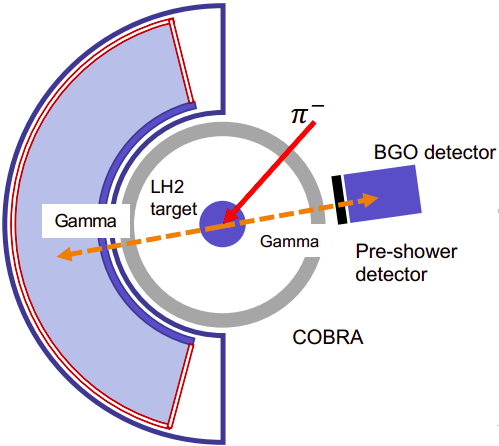
\includegraphics[height=\h, keepaspectratio]{Figures/LH2/CEX_sketch.png}\label{fig:CEX:sketch}}
        \subfloat[BGO crystals]{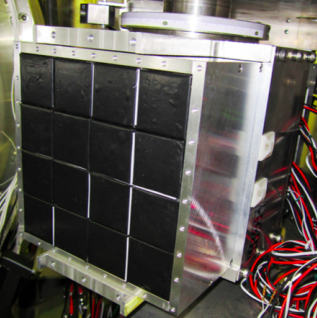
\includegraphics[height=\h]{Figures/LH2/BGO.png}\label{fig:CEX:bgo}}
        \subfloat[BGO mover]{
        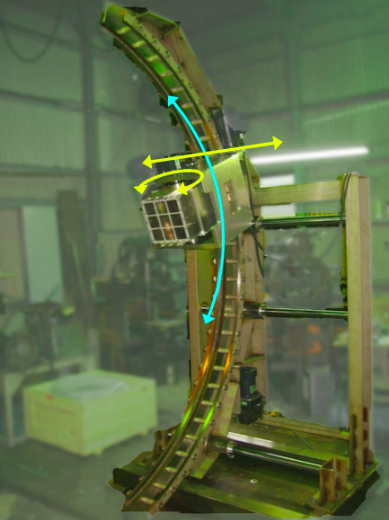
\includegraphics[height=\h, keepaspectratio]{Figures/LH2/BGO_mover.png}\label{fig:CEX:mover}}
        \caption{Diagram of the CEX measurement, with the back-to-back photons configuration to define the XEC patch via the BGO positioning (\ref{fig:CEX:sketch}) Picture of the BGO detector (\ref{fig:CEX:bgo}) Picture of the BGO mover (\ref{fig:CEX:mover}).}
        \label{fig:CEX}
    \end{figure}

\status{review}
\section{BGO}
    \label{sec:LH2:BGO}
    The BGO crystal already mentioned, and shown in Fig.~\ref{fig:CEX:bgo}, is an auxiliary detector that plays a key role in two subjects of this thesis.
    For this reason, we will here describe it in some detail.
    BGO refers to \ce{Bi4Ge3O12}, a compound with a cubic crystal structure and often used as a scintillator.
    This detector is, in particular, a matrix 4x4 of \SI{4x4}{cm} crystals and mounted on a structure (see Fig.~\ref{fig:CEX:mover}) that allows it to translate and rotate around COBRA.
    This detector plays the key role in the back-to-back event tagging but it was also used during the X17 search, subject of Ch.~\ref{ch:X17}.

\status{review}
\section{LH2 target}
    The details of the circuit and the operation changed on a yearly basis but it's worth discussing the overall working principle before seeing the evolution of this system.
    Liquid Hydrogen was chosen to provide the protons needed for the CEX reaction.  
    The incoming 70.6 MeV/c $\pi^-$ are stopped in a cylindrical cell (60 mm diameter, 70 mm length) of 0.5 mm stainless steel containing liquid Hydrogen. 
    This corresponds to $\sim 90\%$ stopping efficiency.
    The hydrogen has to be kept liquid ($T<20.39$ K at 1 atm) and in the center of the COBRA magnet, requiring a cryogenic infrastructure to be inserted for 2 m.
    The target consists of four sub-systems:
    \begin{itemize}
        \item A ``closed volume'' hydrogen circuit, in which a over-pressurized $100\ \ell$ buffer is connected to the target cell 
        \item  A copper rod (2 m in length and 2 cm in diameter): supported and cooled at one end with liquid helium flowing in a copper coil; holding the target cell at the other.
        \item Vacuum Insulation for the whole system
        \item A slow-control based on an SCS2000\footnote{More info can be found here \href{https://daq00.triumf.ca/MidasWiki/index.php/Main_Page}{\underline{MIDAS}} and here \href{https://www.psi.ch/en/ltp-electronics/www-documents}{\underline{SCS and MSCB}}.} for: temperatures, pressures, and He flux
    \end{itemize}
    
    \paragraph{Working principle}
    Let's now outline the working principle of this system.
    The first step is to pressurize with a Helium bottle a Helium dewar.
    When the liquid helium starts flowing in the copper coil, the copper rod is cooled on one side.
    After thermalizing the whole copper rod, the cell temperature slowly follows, reaching the same temperature.
    Once the temperature is low enough for the Hydrogen to condensate, this process in the cell reduces the Hydrogen pressure, sucking additional gas from the buffer.

    \paragraph{The circuit}
    The buffer volume for the gaseous hydrogen, as well as all the infrastructure and services, are kept outside the magnet. The circuit for the 2021 version is shown in Fig. \ref{fig:LH2:2021:circuit} and, to increase the readability, the different sub-circuits are color-coded. 
    Similar sketches are available for the 2022 and 2023 versions, here not shown for simplicity.
    The color coding is kept consistent:
    \begin{itemize}
        \item Blue - Hydrogen is filled into the buffer from a cylinder, which gets then removed.
        The buffer itself is connected to the cell, the exhausting line, a vacuum pump, piezoresistive pressure transmitters and a Nitrogen bottle
        \item Red - The liquid He flux is obtained by pressurizing a Dewar with an He bottle. 
        The He passes around the Cu rod and through a heater before entering the He recovery line
        \item Green - Insulation vacuum system
        \item Yellow - A nitrogen bottle is used for purging the hydrogen when emptying the buffer and kept connected for safety
    \end{itemize}
    

    \begin{sidewaysfigure}
        \centering
        \includegraphics[width=\textwidth]{Figures/LH2/2021/2021_LH2_circuit.png}
        \caption[CEX 2021: LH2 circuit.]{Circuit of the LH2 target. To increase the readability of the scheme of the circuit, the different sub-circuits are color-coded:\\ Blue - Hydrogen; Red - Liquid Helium; Green - Insulation vacuum; Yellow - A nitrogen bottle to flush the system.}
    \label{fig:LH2:2021:circuit}
    \end{sidewaysfigure}

    \status{review}
    \subsection{Operation and control}
        The operation of the target itself is partially manual and partially controlled through a LabVIEW program which, for example, controls the read-out of the various sensors and the flux of the incoming He. 
        A module SCS2000 allows to read the various sensors. 
        There are two key indicators used to monitor the liquefaction process and stability of the system:
    
        \begin{itemize}
            \item Temperature sensors: resistors (later replaced by \lakeshore silicon diodes sensors) have been put in thermal contact with the Cu rod at both ends (two per side for redundancy). 
            The readings of these elements allow us to monitor the cooling at the Cu coil and the cell.
            \item Hydrogen pressure: at room temperature, the hydrogen is set to 1.5 bar over-pressure. When the liquefaction starts the overall pressure is reduced and can be linked to the amount of liquid Hydrogen in the cell. 
        \end{itemize}
        \noindent
        The procedures to operate the system were developed, discussed with the safety committee, and adapted to the different upgrades.
        We will not discuss them here.

\status{started}
\section{2021}
    I started my Ph.D in November 2020 but I joined the activities after the first year, in October 2021. 
    For this reason, I did not participate in the development of the first iteration of the target and I joined directly the tests before the data-taking period.
    The status of the LH2 Target and the preliminary results of the 2021 CEX were presented at the 15th Pisa Meeting on Advanced Detectors \cite{Elba:mio}.

    \status{review}
    \subsection{Data taking}
        The installation process required craning the target in the $\pi E5$ area, on top of a rail system, aligning and inserting the target inside COBRA.
        Pictures of the installation are in Fig.~\ref{fig:CEX:2021:installation}.
        The data taking lasted roughly two weeks, during which CR runs and XEC calibrations were run while the target was cooling and liquefying. 
        As soon as the level was sufficient the pion beam would be used for CEX data taking for a specific patch of the XEC.  
        When the dewar needed to be exchanged, the data taking would be stopped and CR/calibrations would restart, waiting for the target to be sufficiently full to restart.
        \noindent
        In figure \ref{fig:CEX:datataking:2021} is shown the history of the Hydrogen and Helium pressure at the dewar, where the red line marks when the beam was on. 
        Interesting features are:
        \begin{outline}
            \1 The decreasing parts of the blue plot are the liquefaction period: the Hydrogen pressure drops because of the phase change
            \1 During liquefaction, some spikes can be seen: these are instances in which the system became unstable and liquefaction was lost
            \1 The speed of cooling and liquefaction is always the same, a result of hardware 
        \end{outline}
        Overall, CEX data could be collected when the target was considered `full enough': below 2.1 bar, meaning 50\% full. 
        In the two weeks, this translates to efficiency of $D_{2021}\approx0.5$.
        The efficiency for 2021 was lower than expected and the necessary statistic was not reached for every patch (Fig.~\ref{fig:CEX:patches:2021}).

        \begin{figure}
            \centering
            \subfloat[The target in the testing area, before the craning.]{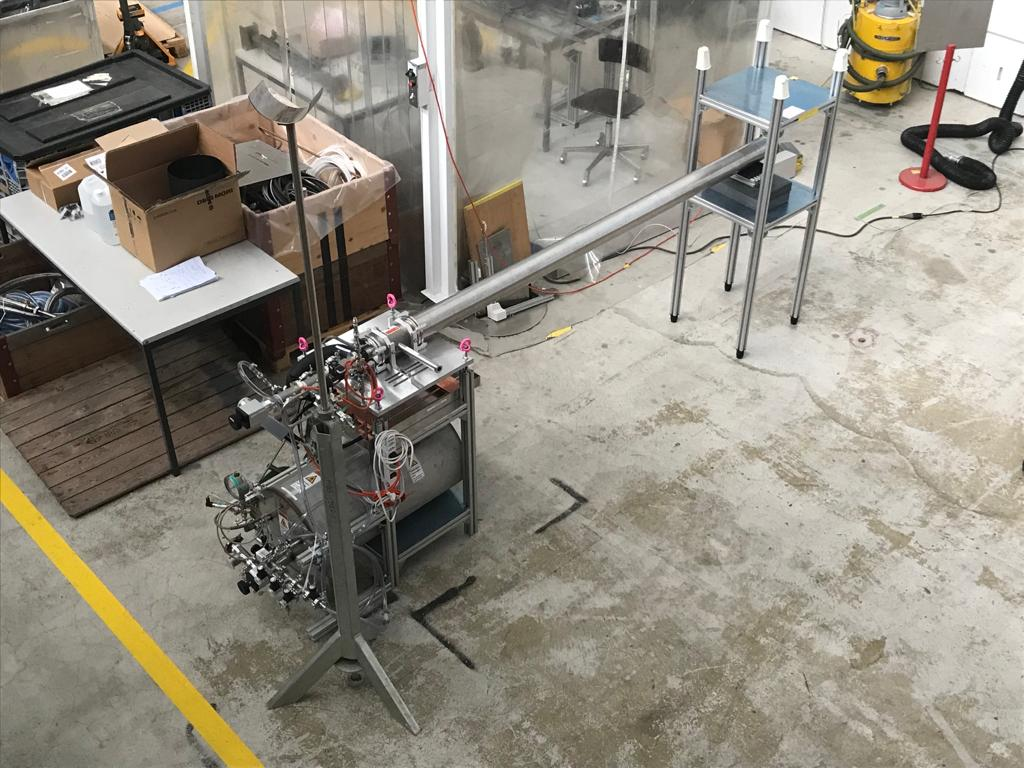
\includegraphics[height =  6cm, keepaspectratio]{Figures/LH2/2021/CEX2021_out.jpg}}
            \subfloat[Target after the insertion in COBRA]{
            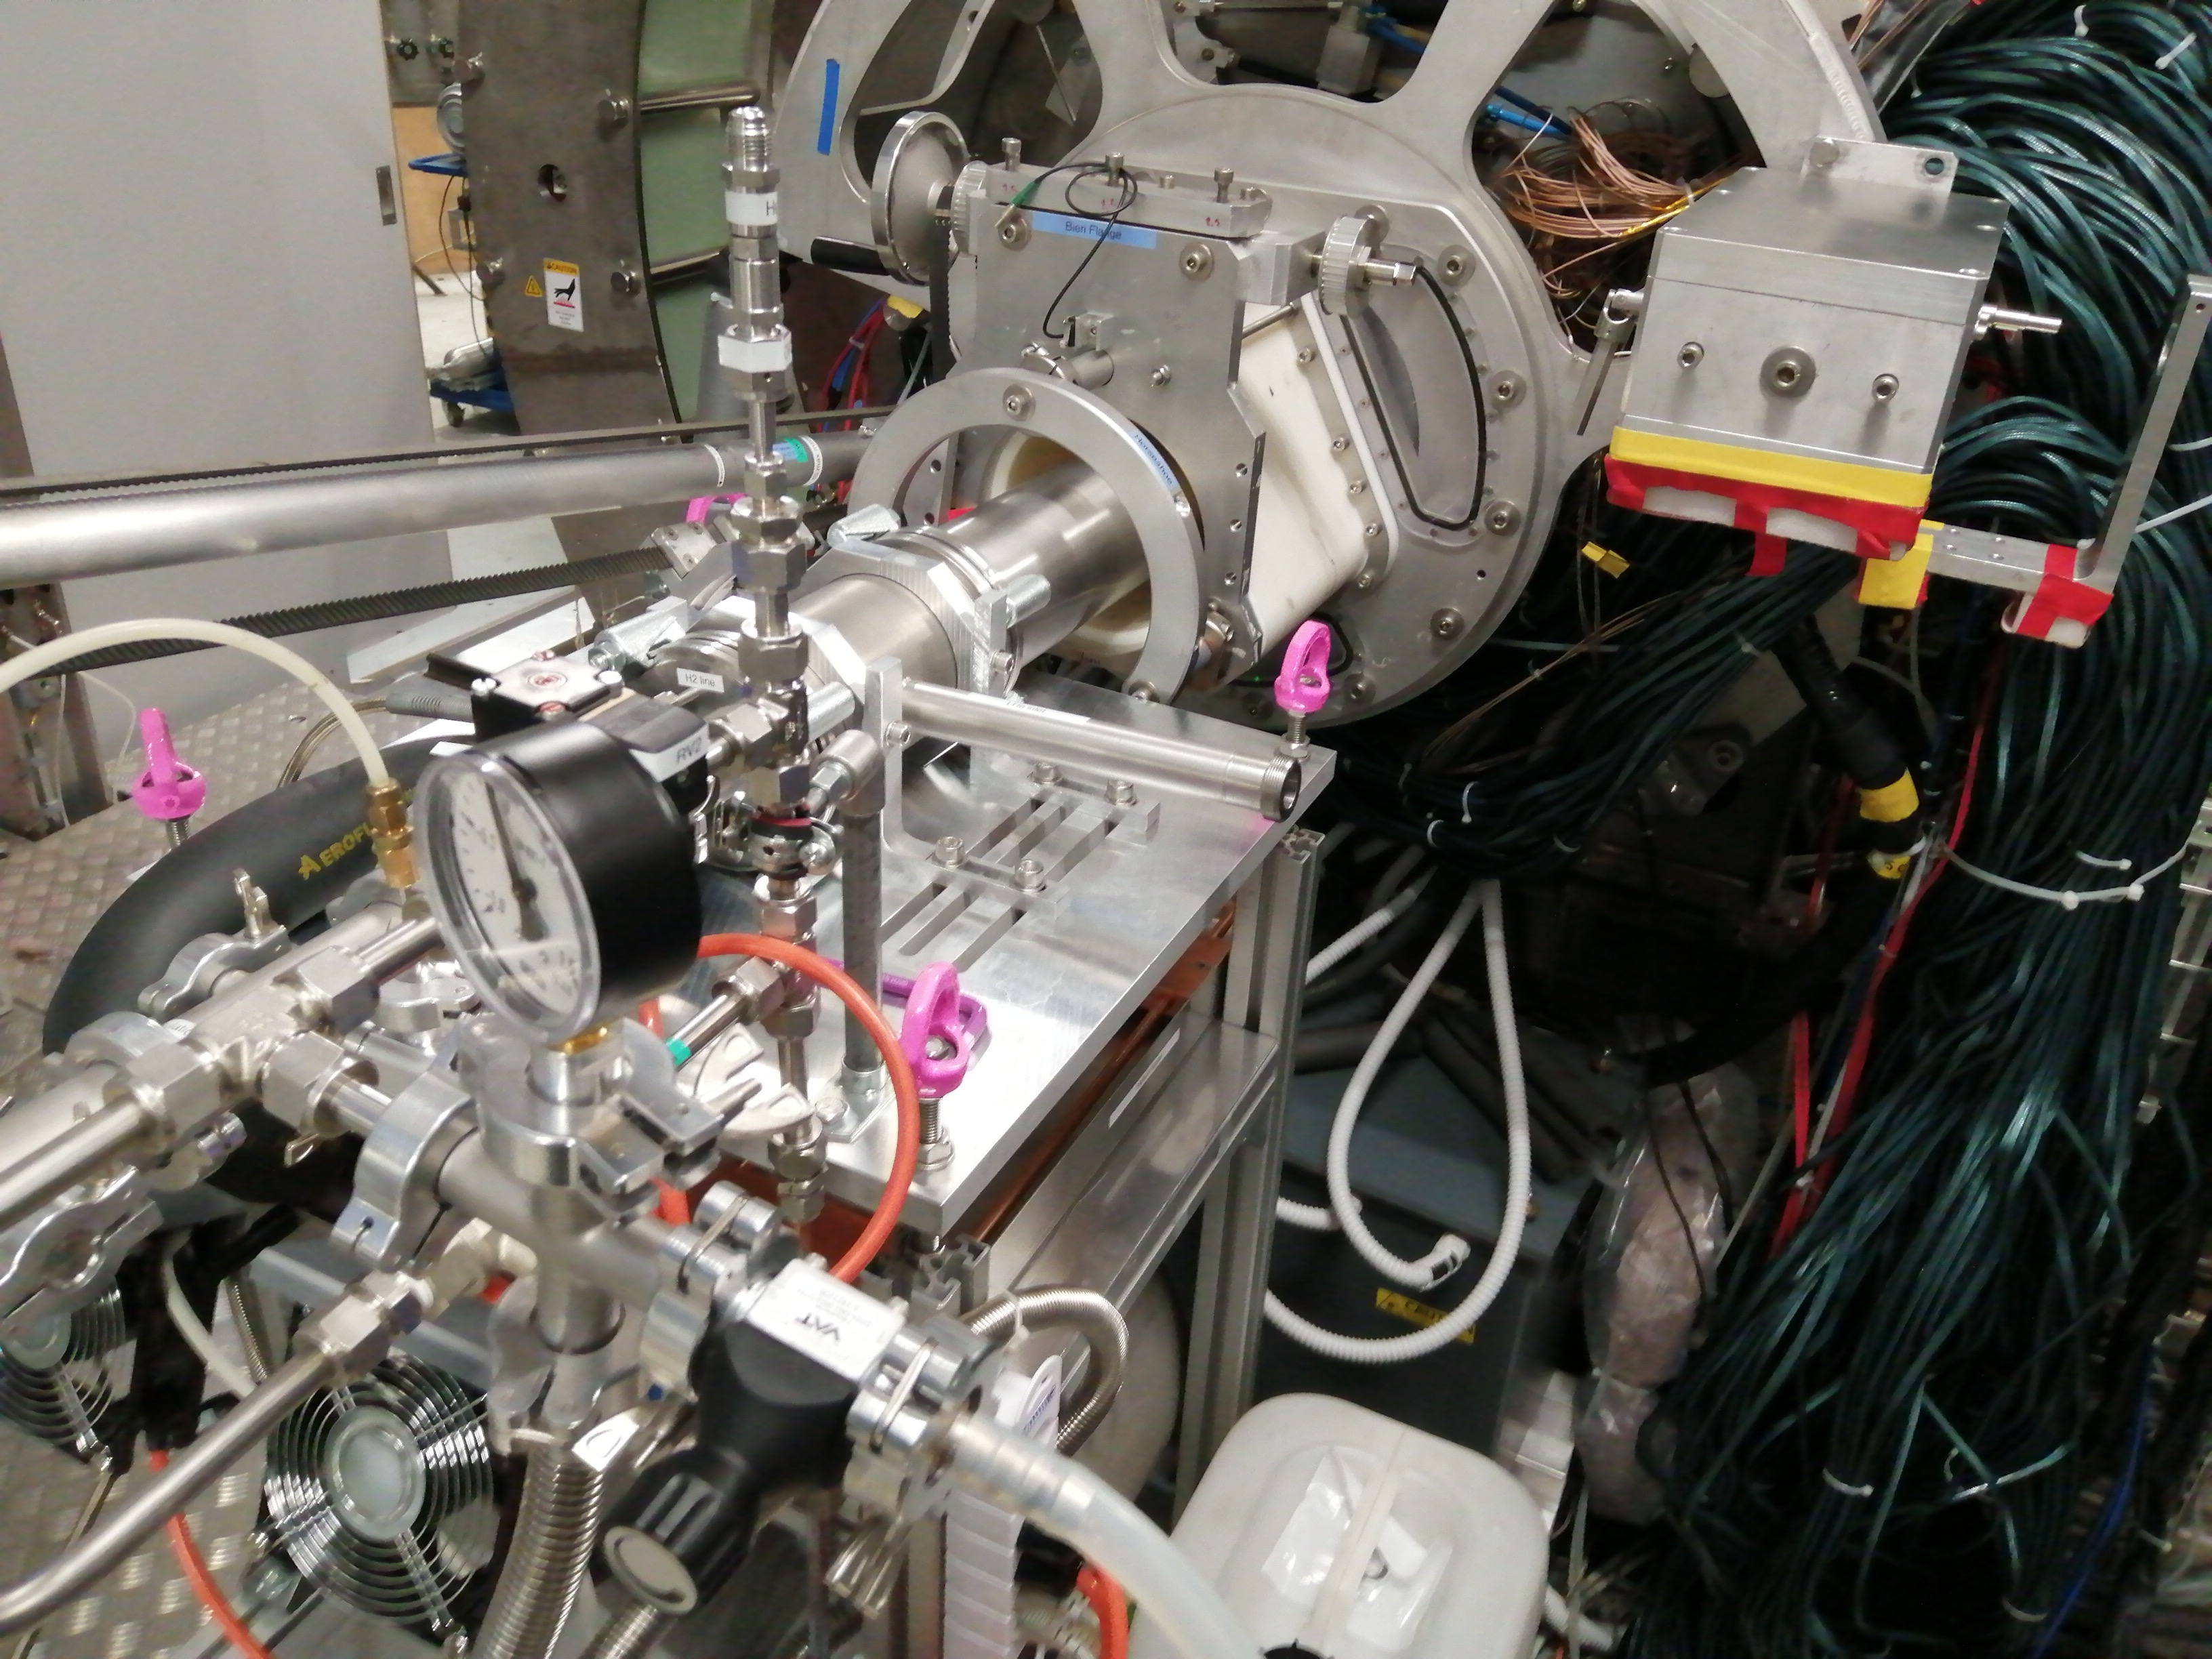
\includegraphics[height = 6cm, keepaspectratio]{Figures/LH2/2021/XEC2021_inserted.jpeg}}
            \caption{Pictures of the Liquid Hydrogen target outside $\pi E5$ and after the insertion in COBRA.}
            \label{fig:CEX:2021:installation}
        \end{figure}

    \status{started}
    \subsection{Data anlaysis}
        While the broad idea of the XEC calibrations was already outlined in Sec.~\ref{sec:MEG:XEC}, it is perhaps worth now describing how the analysis of the data from the Carge EXchange reaction allows extracting not only the timing and energy resolution but also the energy scale.
        
        \paragraph{Timing}
        The time resolution of the XEC was evaluated by taking the difference in time between the detector and the pre-shower counter, correcting for the time of flight (TOF).
        \begin{align}
            \Delta t &= t_\g - t_{ps} - t_{TOF}\\
            \sigma_{\Delta t} &=  \sigma_{t_\g} \oplus \sigma_{t_{ps}} \oplus \sigma_{t_{TOF}}
        \end{align}
        The contribution coming from the pre-shower counter, , being it comprised of scintillators, was measured and found to be $\sigma_{ps}=\SI{28.2(2)}{ns}$.
        The main contribution to $\sigma_{t_{TOF}}$ comes from the resolution in the position of the vertex $\sigma_{vertex}$.
        This can be evaluated as 
        $$\sigma_{t_{vertex}} = \sigma_{vertex} \oplus \sigma_{ref} \oplus \sigma_{ps}$$
        Due to the reduce statistics, the result was $\sigma_{verted} = \SI{70(6)}{ps}$.
        Adding the measured $\sigma_{\Delta t} = \SI{99.5(5)}{ps}$, we have all the elements to extract the intrinsic resolution of the detector.
        The timing resolution found is energy-dependent as well as position-dependent, but, for the interesting range $\SI{50}{MeV}<E_\gamma<\SI{58}{MeV}$ and with minimal cut, the result is $\sigma_{t_\g}=\SI{65(6)}{ps}$, as shown in Fig.~\ref{fig:CEX:2021:timing}. 

        \begin{figure}
            \centering
            \subfloat[Scheme with reference counter and pre-shower.]{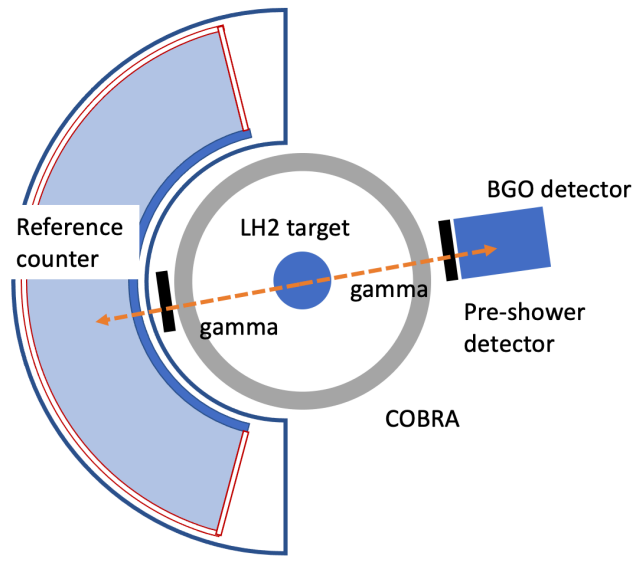
\includegraphics[height = 5cm, keepaspectratio]{Figures/LH2/2021/CEX_preshower_reference.png}}
            \subfloat[Extracted timing resolution from CEX 2021.]{
            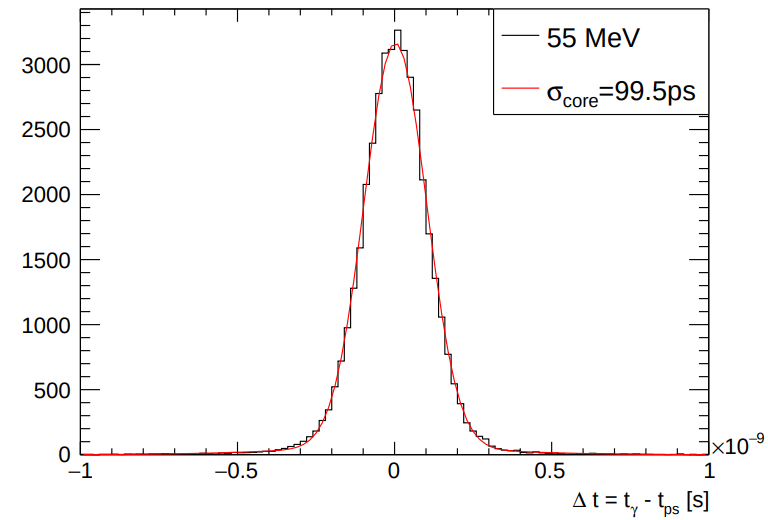
\includegraphics[height = 5cm, keepaspectratio]{Figures/LH2/2021/CEX2021_time.png}}
            \caption{}
            \label{fig:CEX:2021:timing}
        \end{figure}

        \begin{figure}
            \centering
            \subfloat[Number of event per patch during CEX 2021]{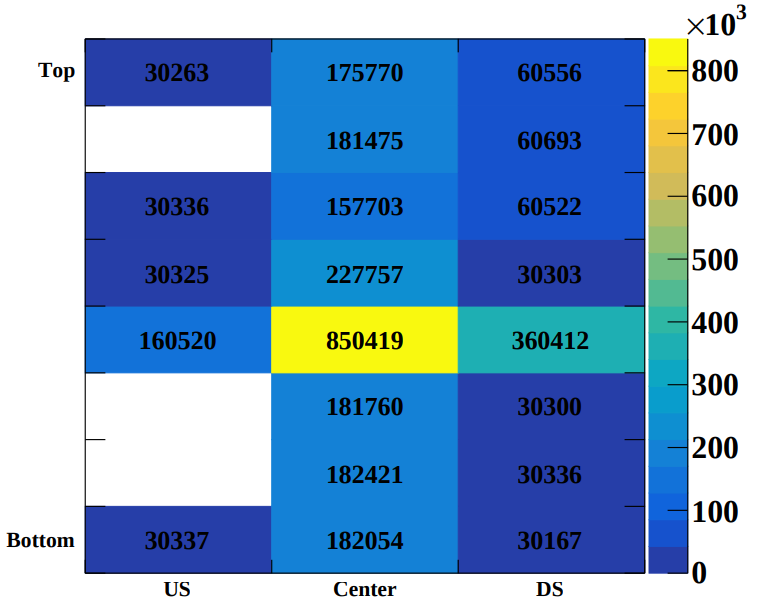
\includegraphics[height = 5cm, keepaspectratio]{Figures/LH2/2021/CEX2021_patches.png}}
            \subfloat[E]{
            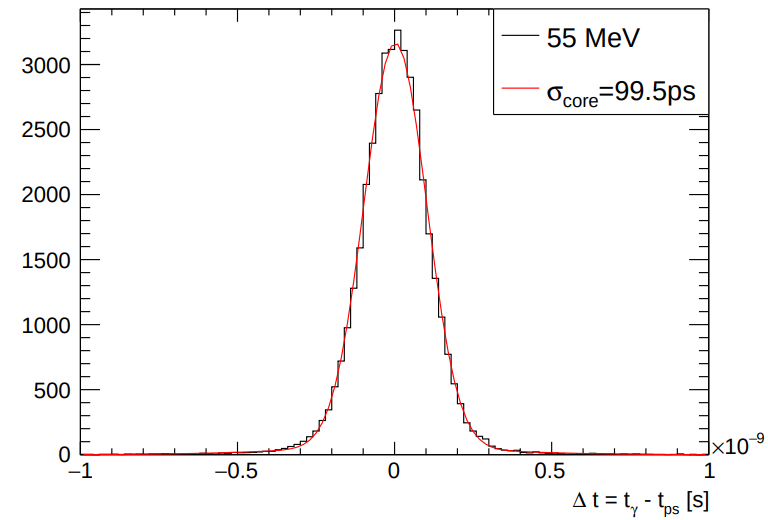
\includegraphics[height = 5cm, keepaspectratio]{Figures/LH2/2021/CEX2021_time.png}}
            \caption{}
            \label{fig:CEX:2021:energy}
        \end{figure}

        \paragraph{Energy} The data collected during the CEX have been used for two purposes: as one of the points in the evaluation of the resolution in the energy of the detector and to evaluate the absolute scaling of the energy measured.
        
\status{review}
\section{2022}
    After (the only partial success of) the 2021 CEX data-taking, major upgrades were needed.
    We modified key aspects of the target and managed to test it before moving it to the experimental area.
    This step was not possible in 2021 because of safety regulations around the usage of Hydrogen.

    \status{review}
    \subsection{Upgrades}
        \paragraph{He circuit} The liquid helium circuit of the 2021 version had a  design flow, namely the `output' from the target was not under vacuum.
        This was solved by adding a section to the back side of the target, similar in design to the `inlet`: a beam pipe part on which an evacuated pipe was soldered such that the nozzle of the transfer line could be connected.
        A picture of the outlet part is in Fig.~\ref{fig:CEX:2022:insulation}.
        
        \paragraph{Cell} Another problem of the previous design was the fact that the thermal contact between the cold copper rod and the cell was through a thick wall of stainless steel. 
        The material is a requirement for the safe use of hydrogen, but the thickness of the back wall of the cell was excessive.
        The result was that, even with a very cold copper rod, this thermal contact was not enough to contrast the heat load of the cell itself.
        The upgraded version has a few differences from the previous one:
        \begin{outline}
            \1 The base of the cell has a thinner wall in correspondence to the copper rod, to improve the thermal contact. The thickness was chosen to be AAA \SI{}{mm}.
            \1 This part is brazed to a threaded copper cylinder, this allows the cell to be mounted and dismounted if needed. 
            Another advantage is that, if the thermal connection is achieved, the surface for heat exchange is increased.
        \end{outline}
        A sketch of the design and a picture of the resulting cell are in Fig.~\ref{fig:CEX:2022:cell}
        
        \paragraph{Shielding} To improve the stability of the system and the thermal load due to the radiation of the vacuum pipe to the cold system, two types of shielding were introduced:
        \begin{outline}
            \1 A copper sheet was bent to create an intermediate cylinder between the main copper rod and the vacuum pipe. The reason is to have this shield to an intermediate temperature and reduce the thermal radiation of the system. 
            \1 Multi-layer insulation\footnote{This type of insulation is standard in cryogenic infrastructure, for example, it is used in liquid helium dewars.} on the helium line, the main copper rod, and the hydrogen line. This insulation is made of alternated layers of thin metal and plastic `nets' to create concentric layers at different temperatures. 
        \end{outline}
        Pictures of the target after adding these shieldings are in Fig.~\ref{fig:CEX:2022:insulation}. 

        \paragraph{Sensors} The PT100 sensors used in 2021 were not suited for very low-temperature readings but were used due to time constraints. 
        For this reason in 2022, we added two additional sensors\footnote{For additional info visit the \href{https://www.lakeshore.com/products/categories/overview/temperature-products/cryogenic-temperature-sensors/germanium}{\underline{\lakeshore}} website.} from \lakeshore.
        These new sensors have been screwed on the copper rod with a ring of Indium to improve the thermal connection. 
        A picture of a mounting test of such a sensor and the additional relative feedthrough are in Fig.~\ref{fig:CEX:2022:sensors}.

        \begin{figure}
            \centering
            \subfloat[Design of the new cell.]{
            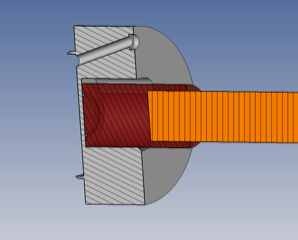
\includegraphics[height = 6cm, keepaspectratio]{Figures/LH2/2022/CEX2022_celldesign.png}}
            \hfill
            \subfloat[Picture of the parts before brazing.]{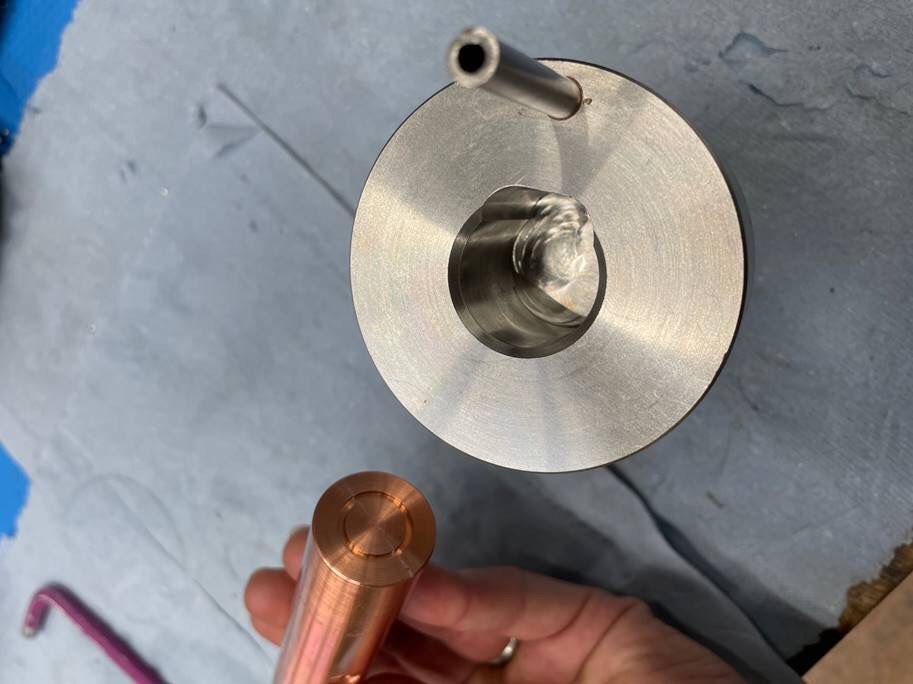
\includegraphics[height =  6cm, keepaspectratio]{Figures/LH2/2022/CEX2022_cell.jpeg}}
            \caption{A new cell was designed to be faster in the cooling/liquefaction and mountable.}
            \label{fig:CEX:2022:cell}
        \end{figure}
        
        \begin{figure}
            \centering
            \subfloat[A test of the mounting procedure.]{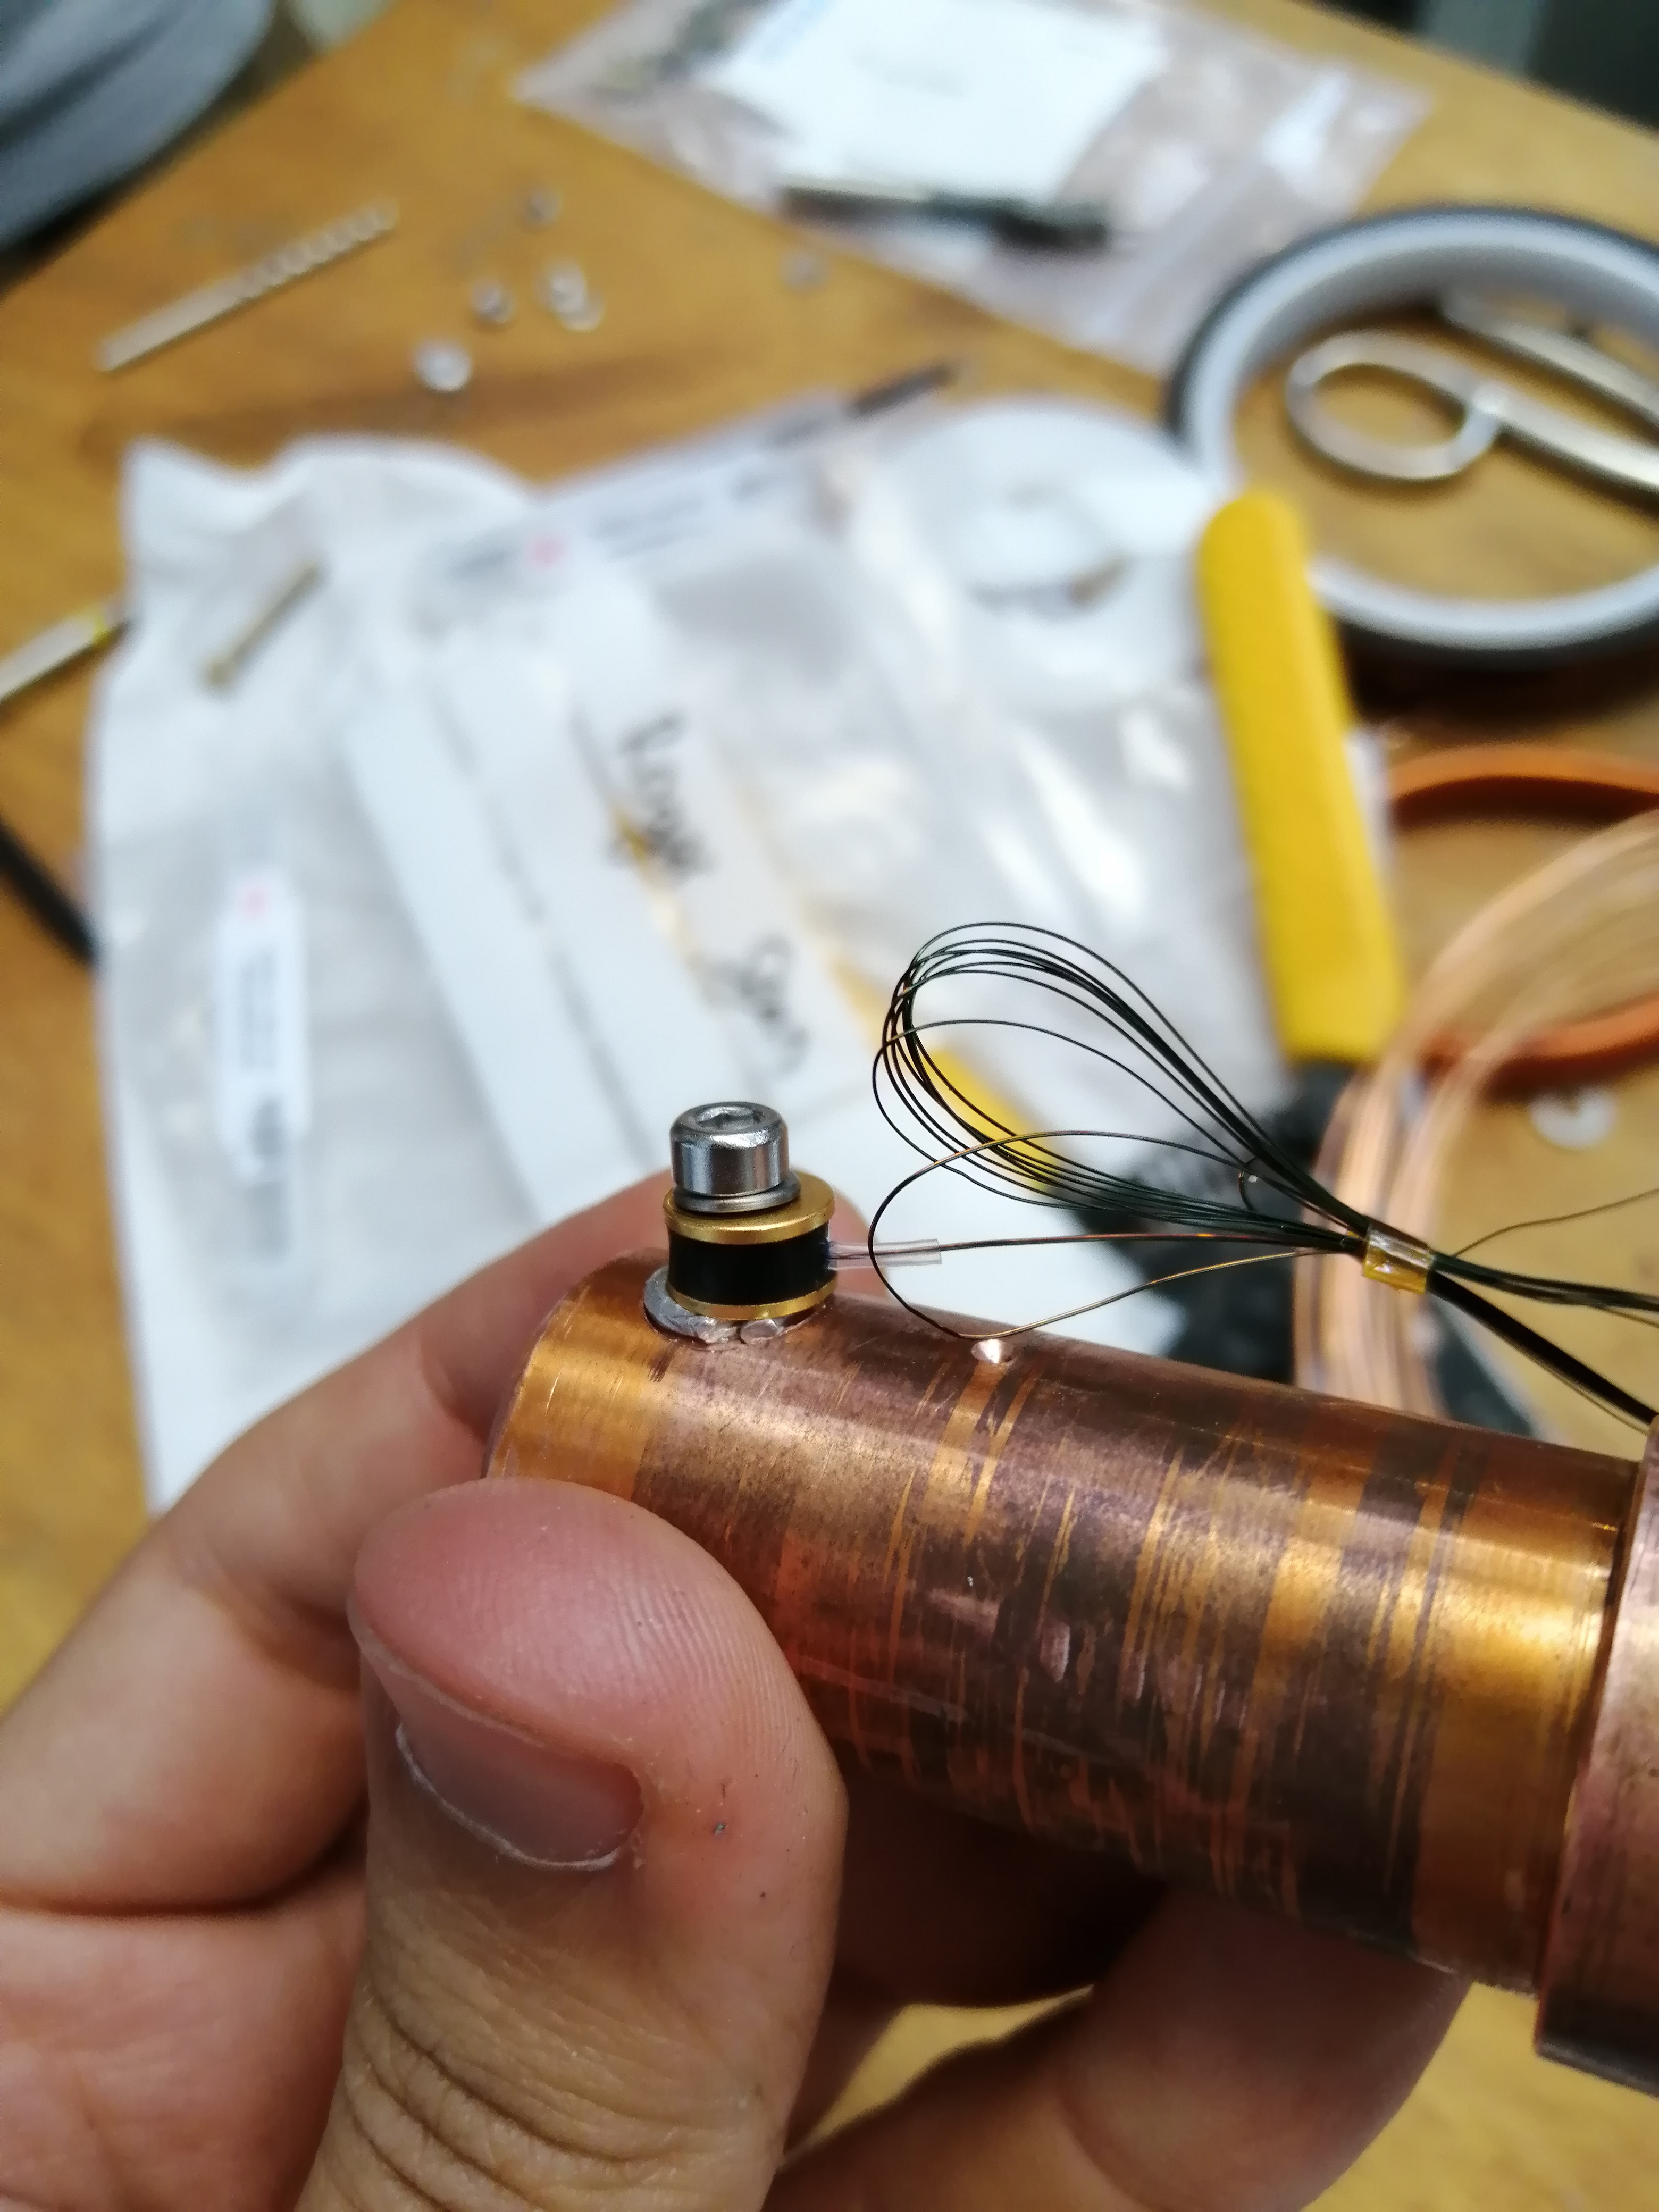
\includegraphics[height =  10cm, keepaspectratio]{Figures/LH2/2022/CEX2022_lakeshores.jpg}}
            \hfill
            \subfloat[Additional feedthrough were soldered.]{
            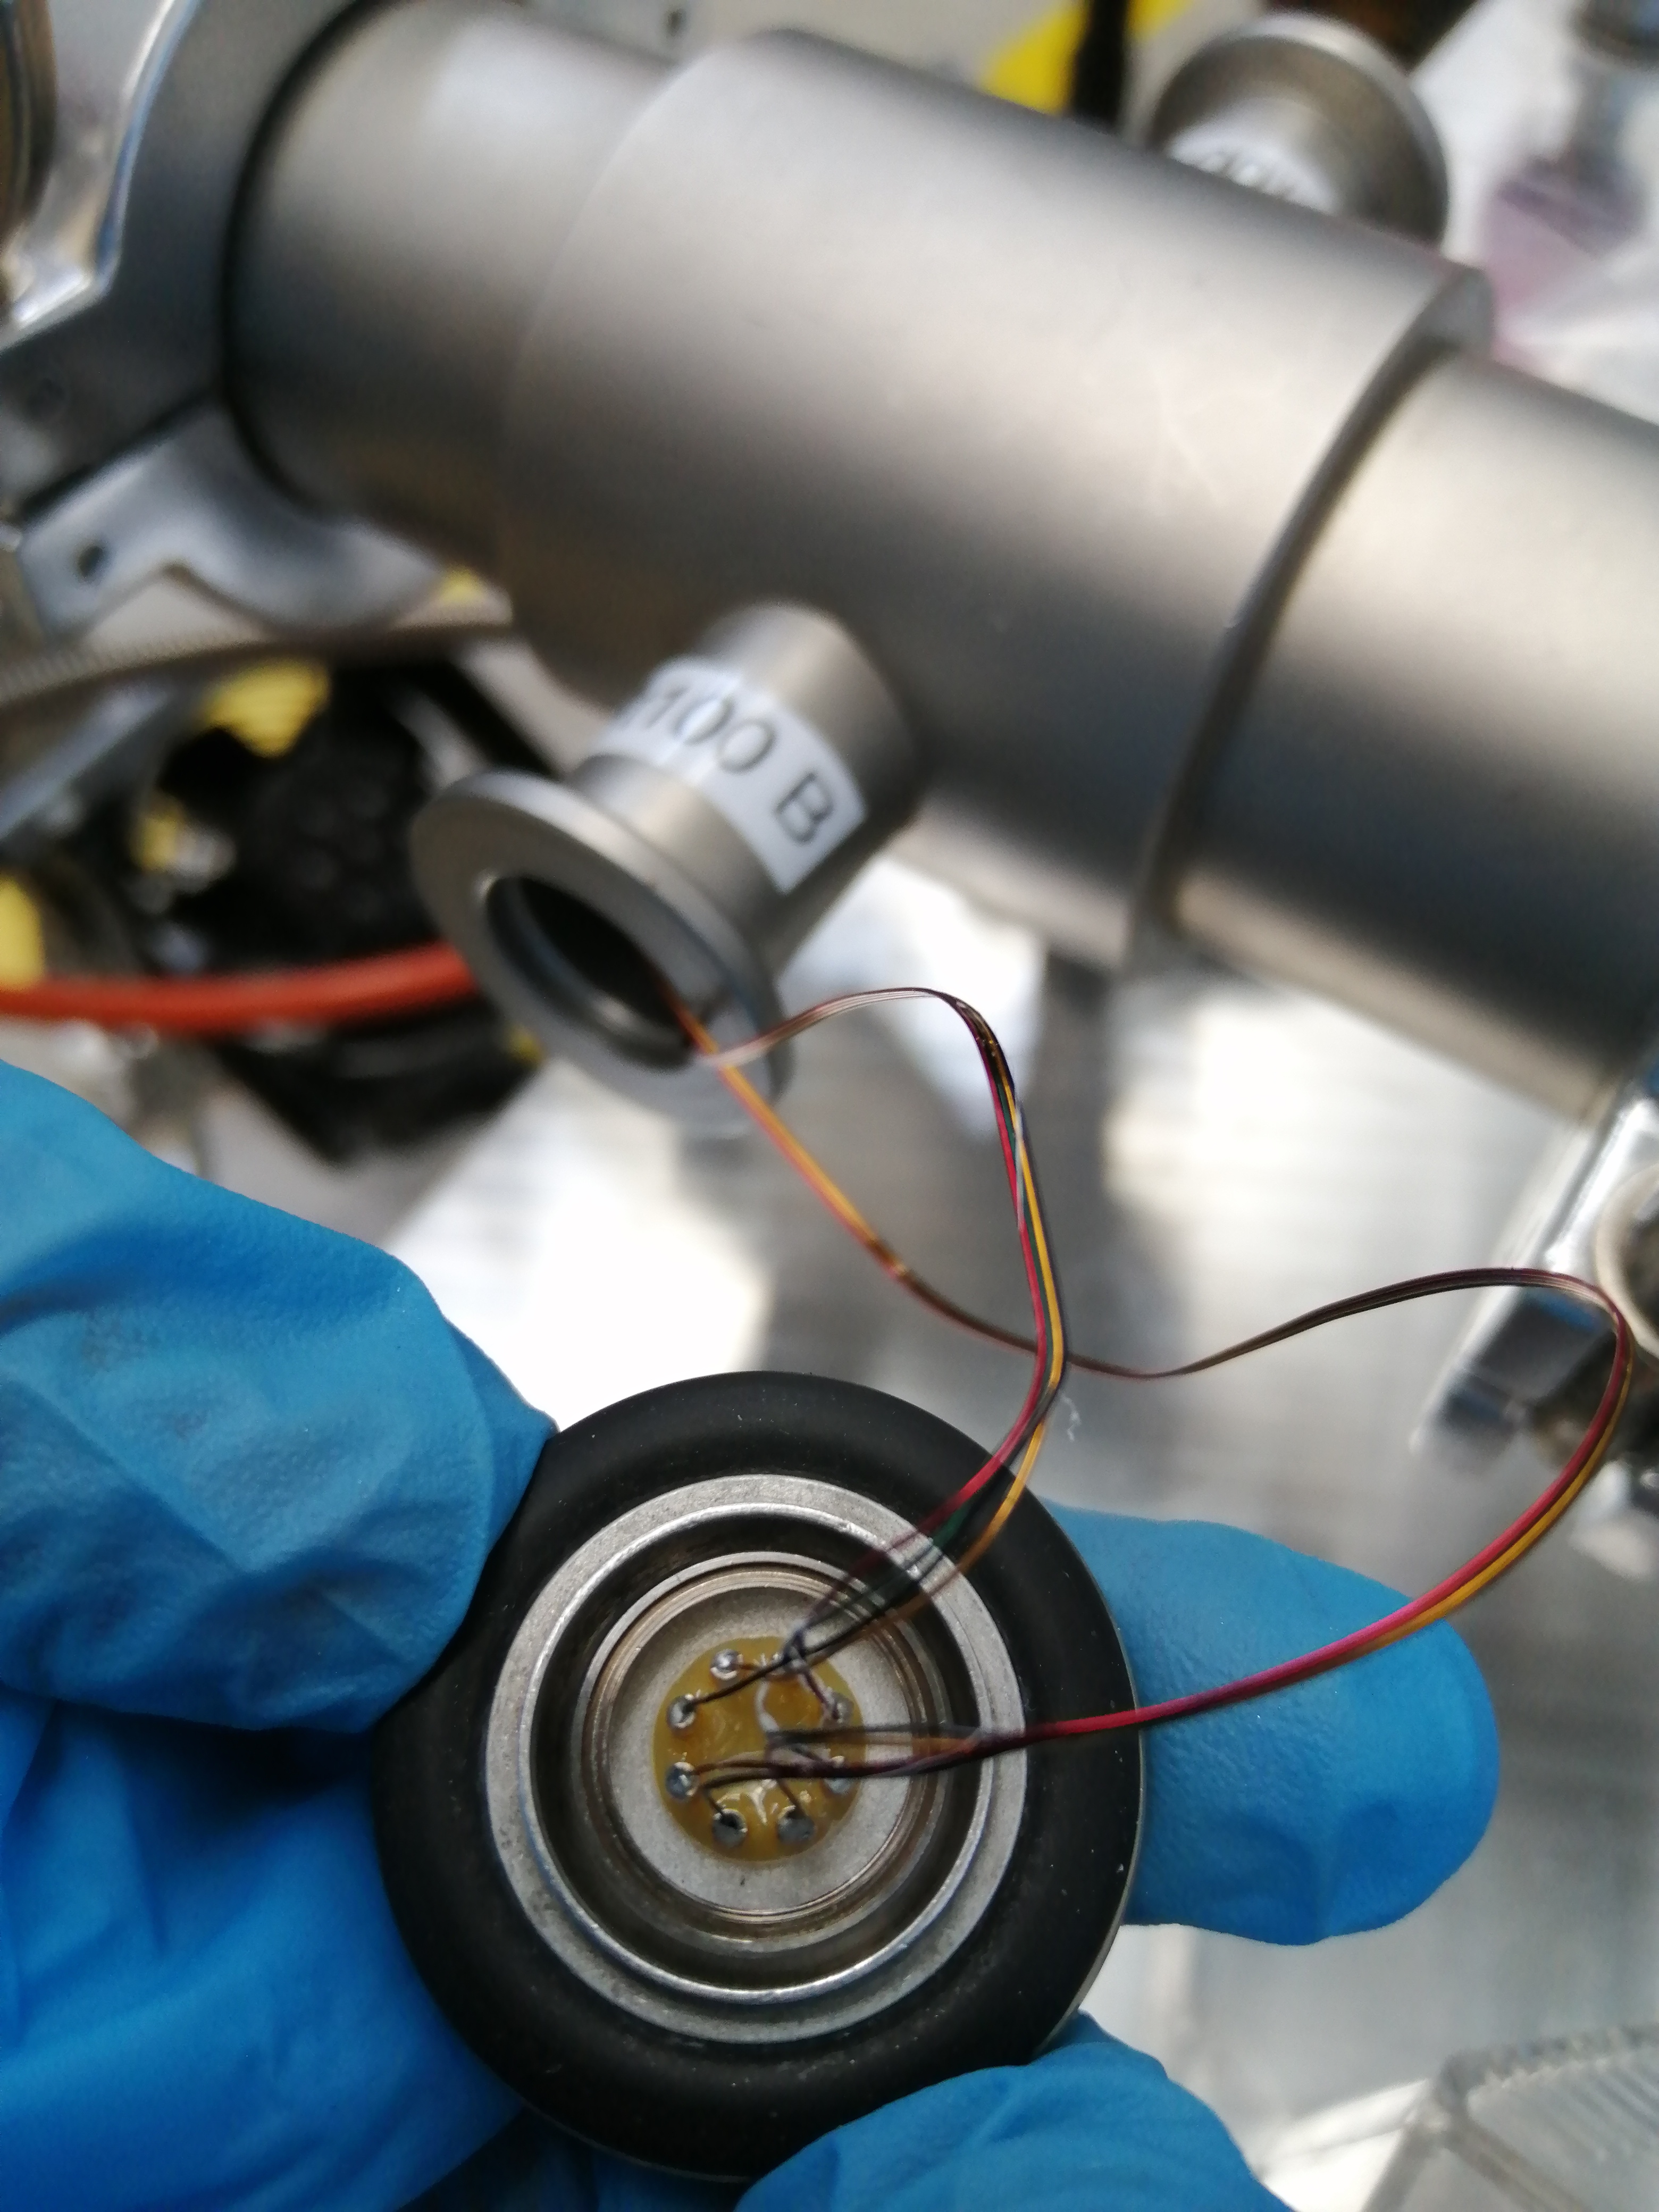
\includegraphics[height = 10cm, keepaspectratio]{Figures/LH2/2022/CEX2022_feedthrough.jpg}}
            \caption{Pictures taken while mounting the \lakeshore sensors.}
            \label{fig:CEX:2022:sensors}
        \end{figure}

        \begin{figure}
            \centering
            
            \subfloat[Multi-layer superinsulation was added.]{
            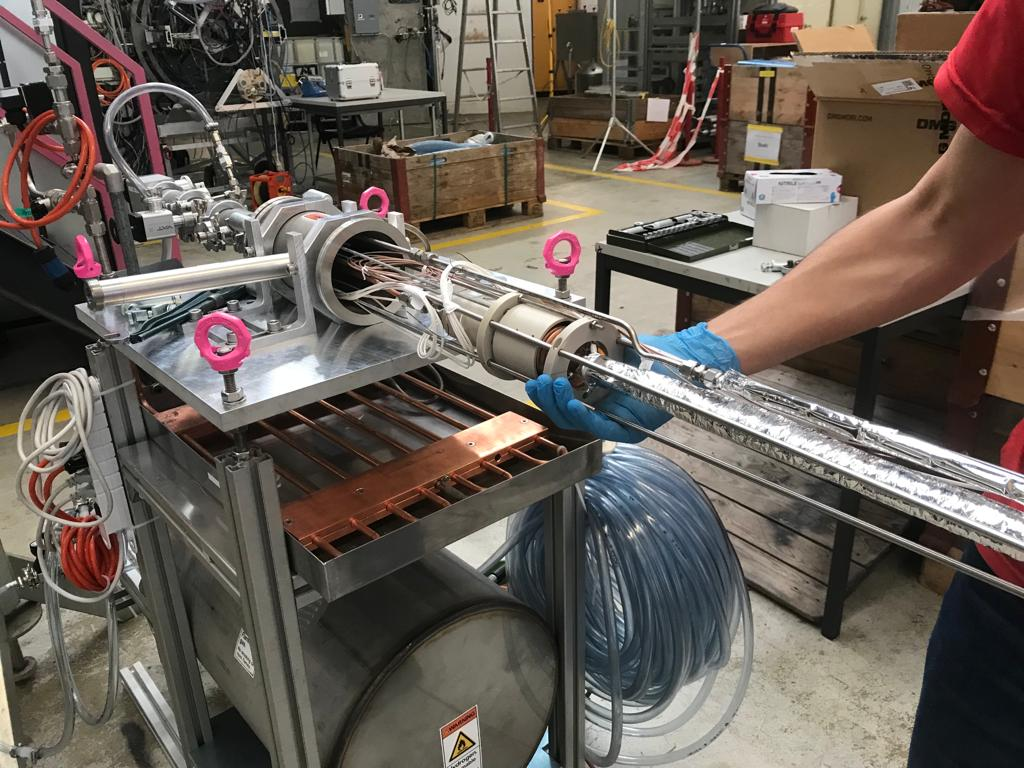
\includegraphics[height = 10cm, keepaspectratio]{Figures/LH2/2022/CEX2022_superinsulation.jpg}}\\
            \subfloat[A vacuumed outlet was designed.]{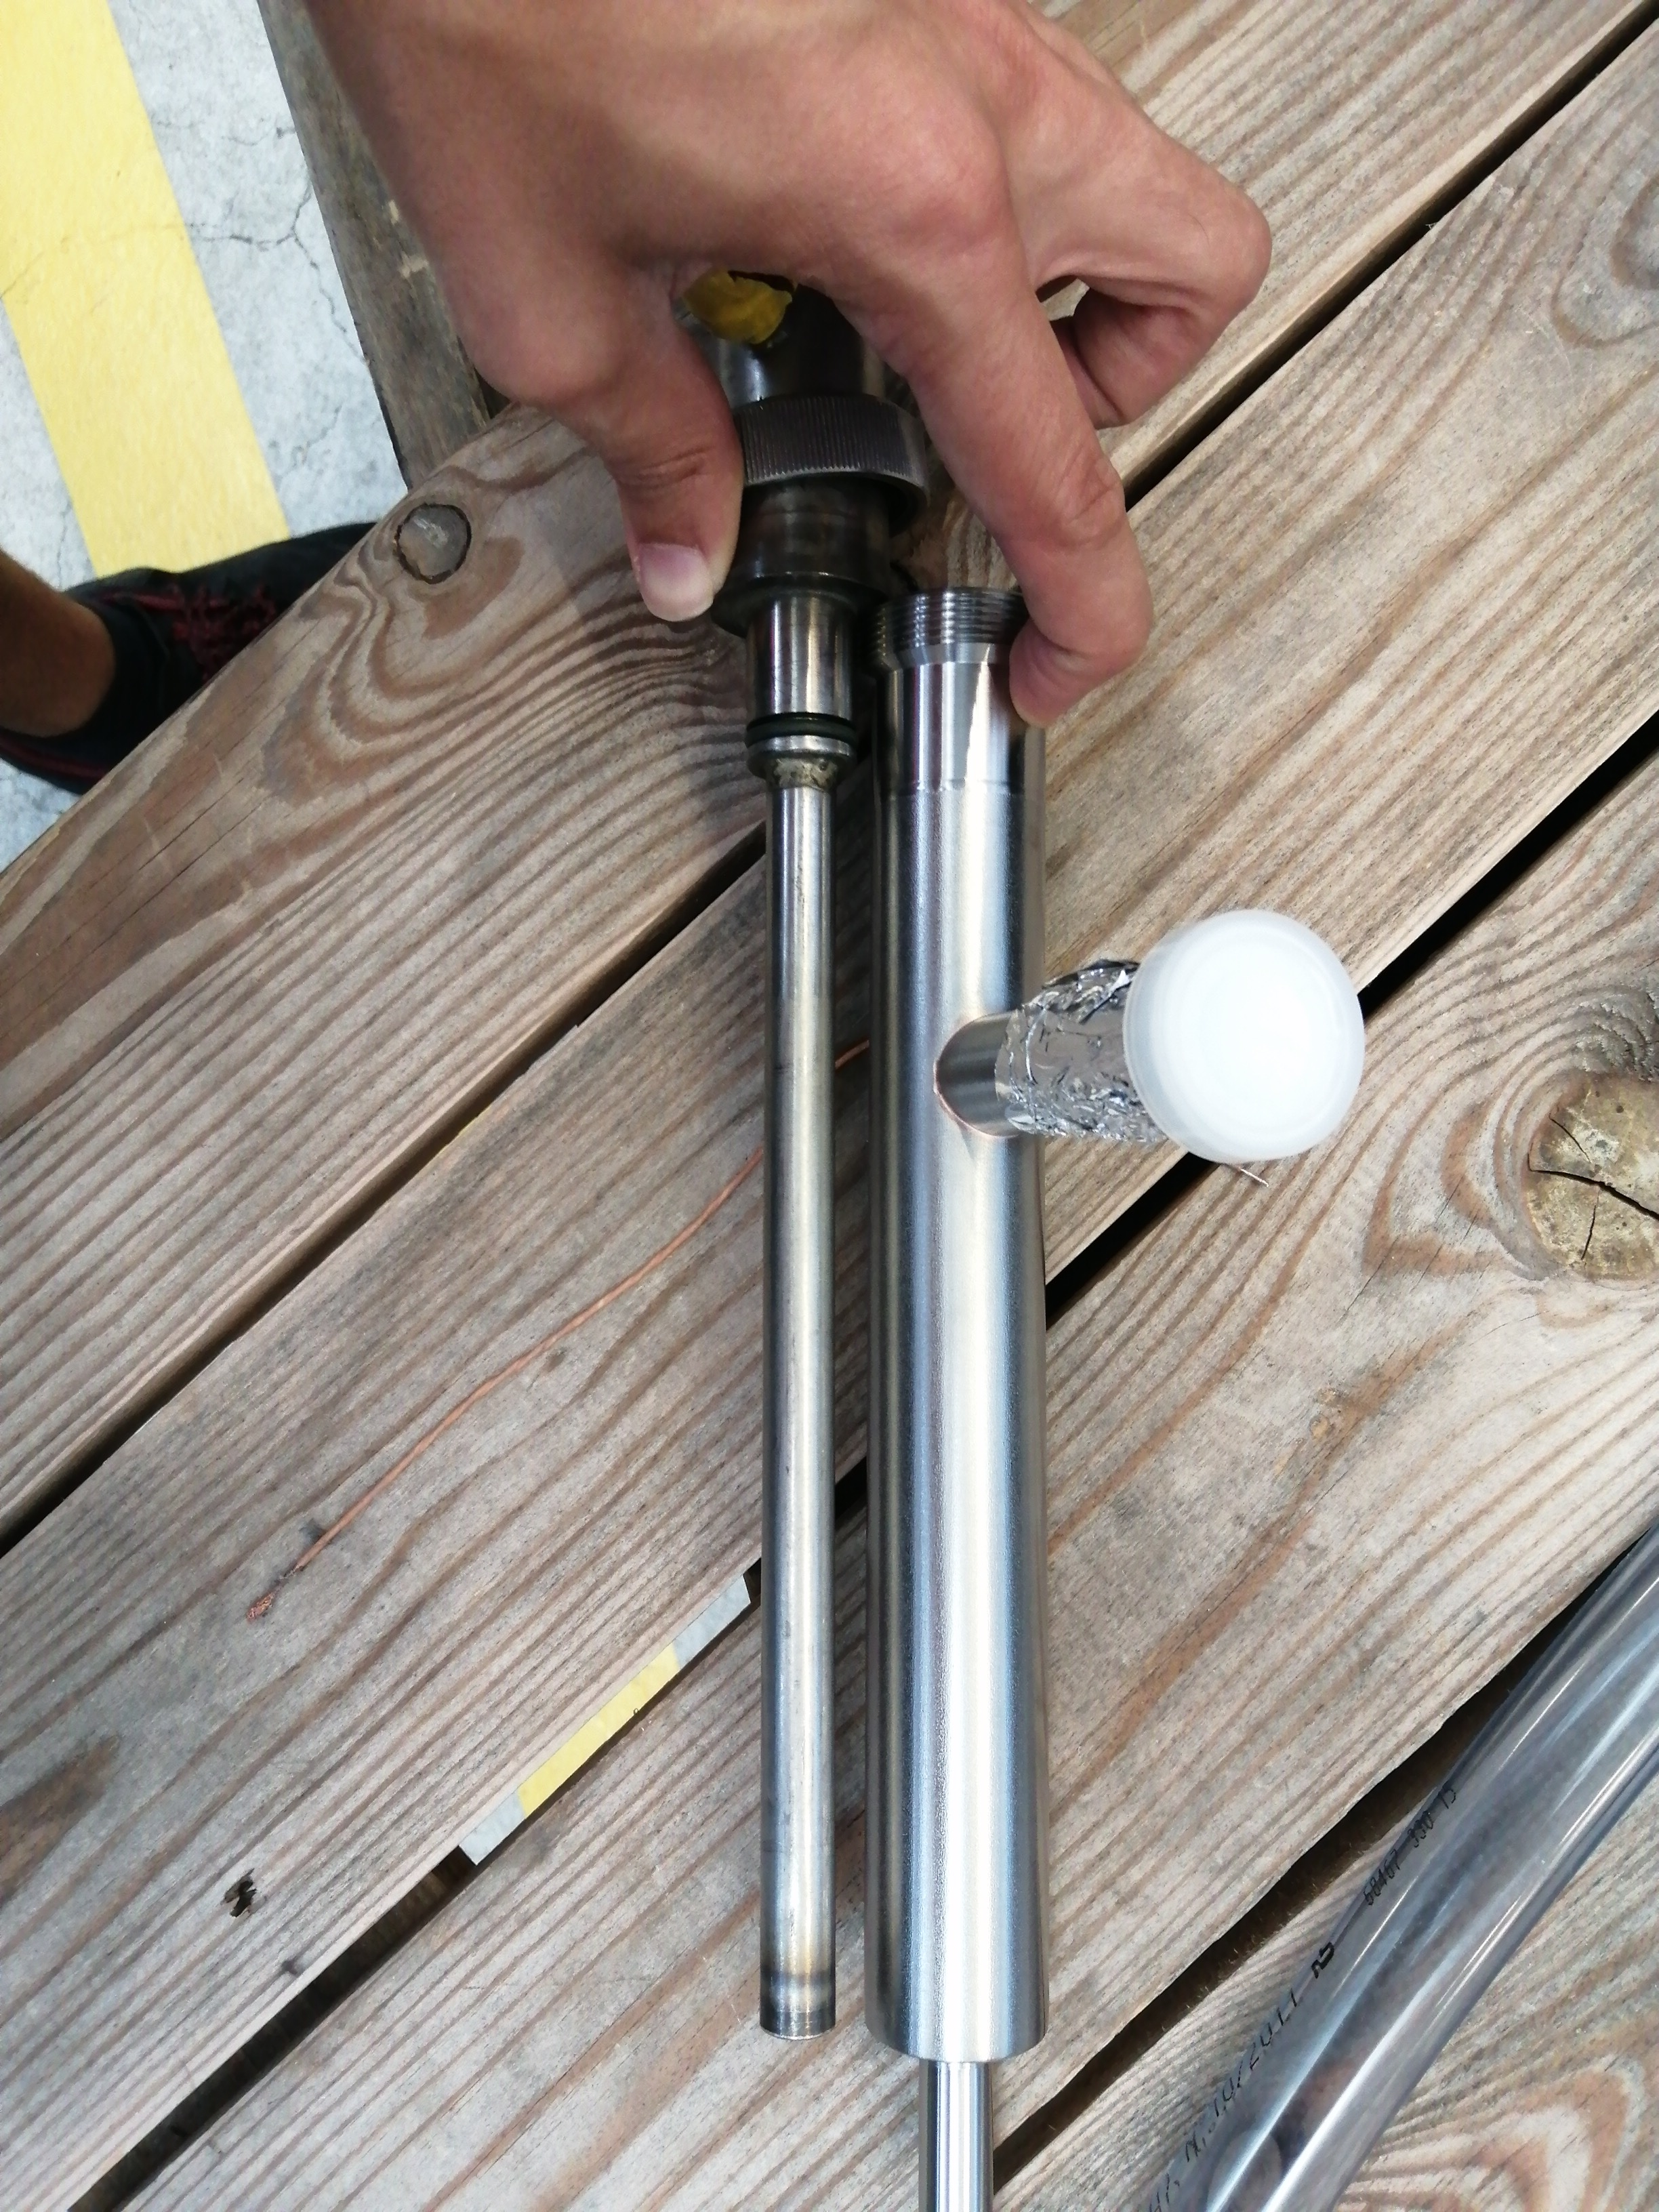
\includegraphics[height =  10cm, keepaspectratio]{Figures/LH2/2022/CEX2022_outlet.jpeg}}
            \hfill
            \subfloat[Shieldig was added around the whole structure.]{
            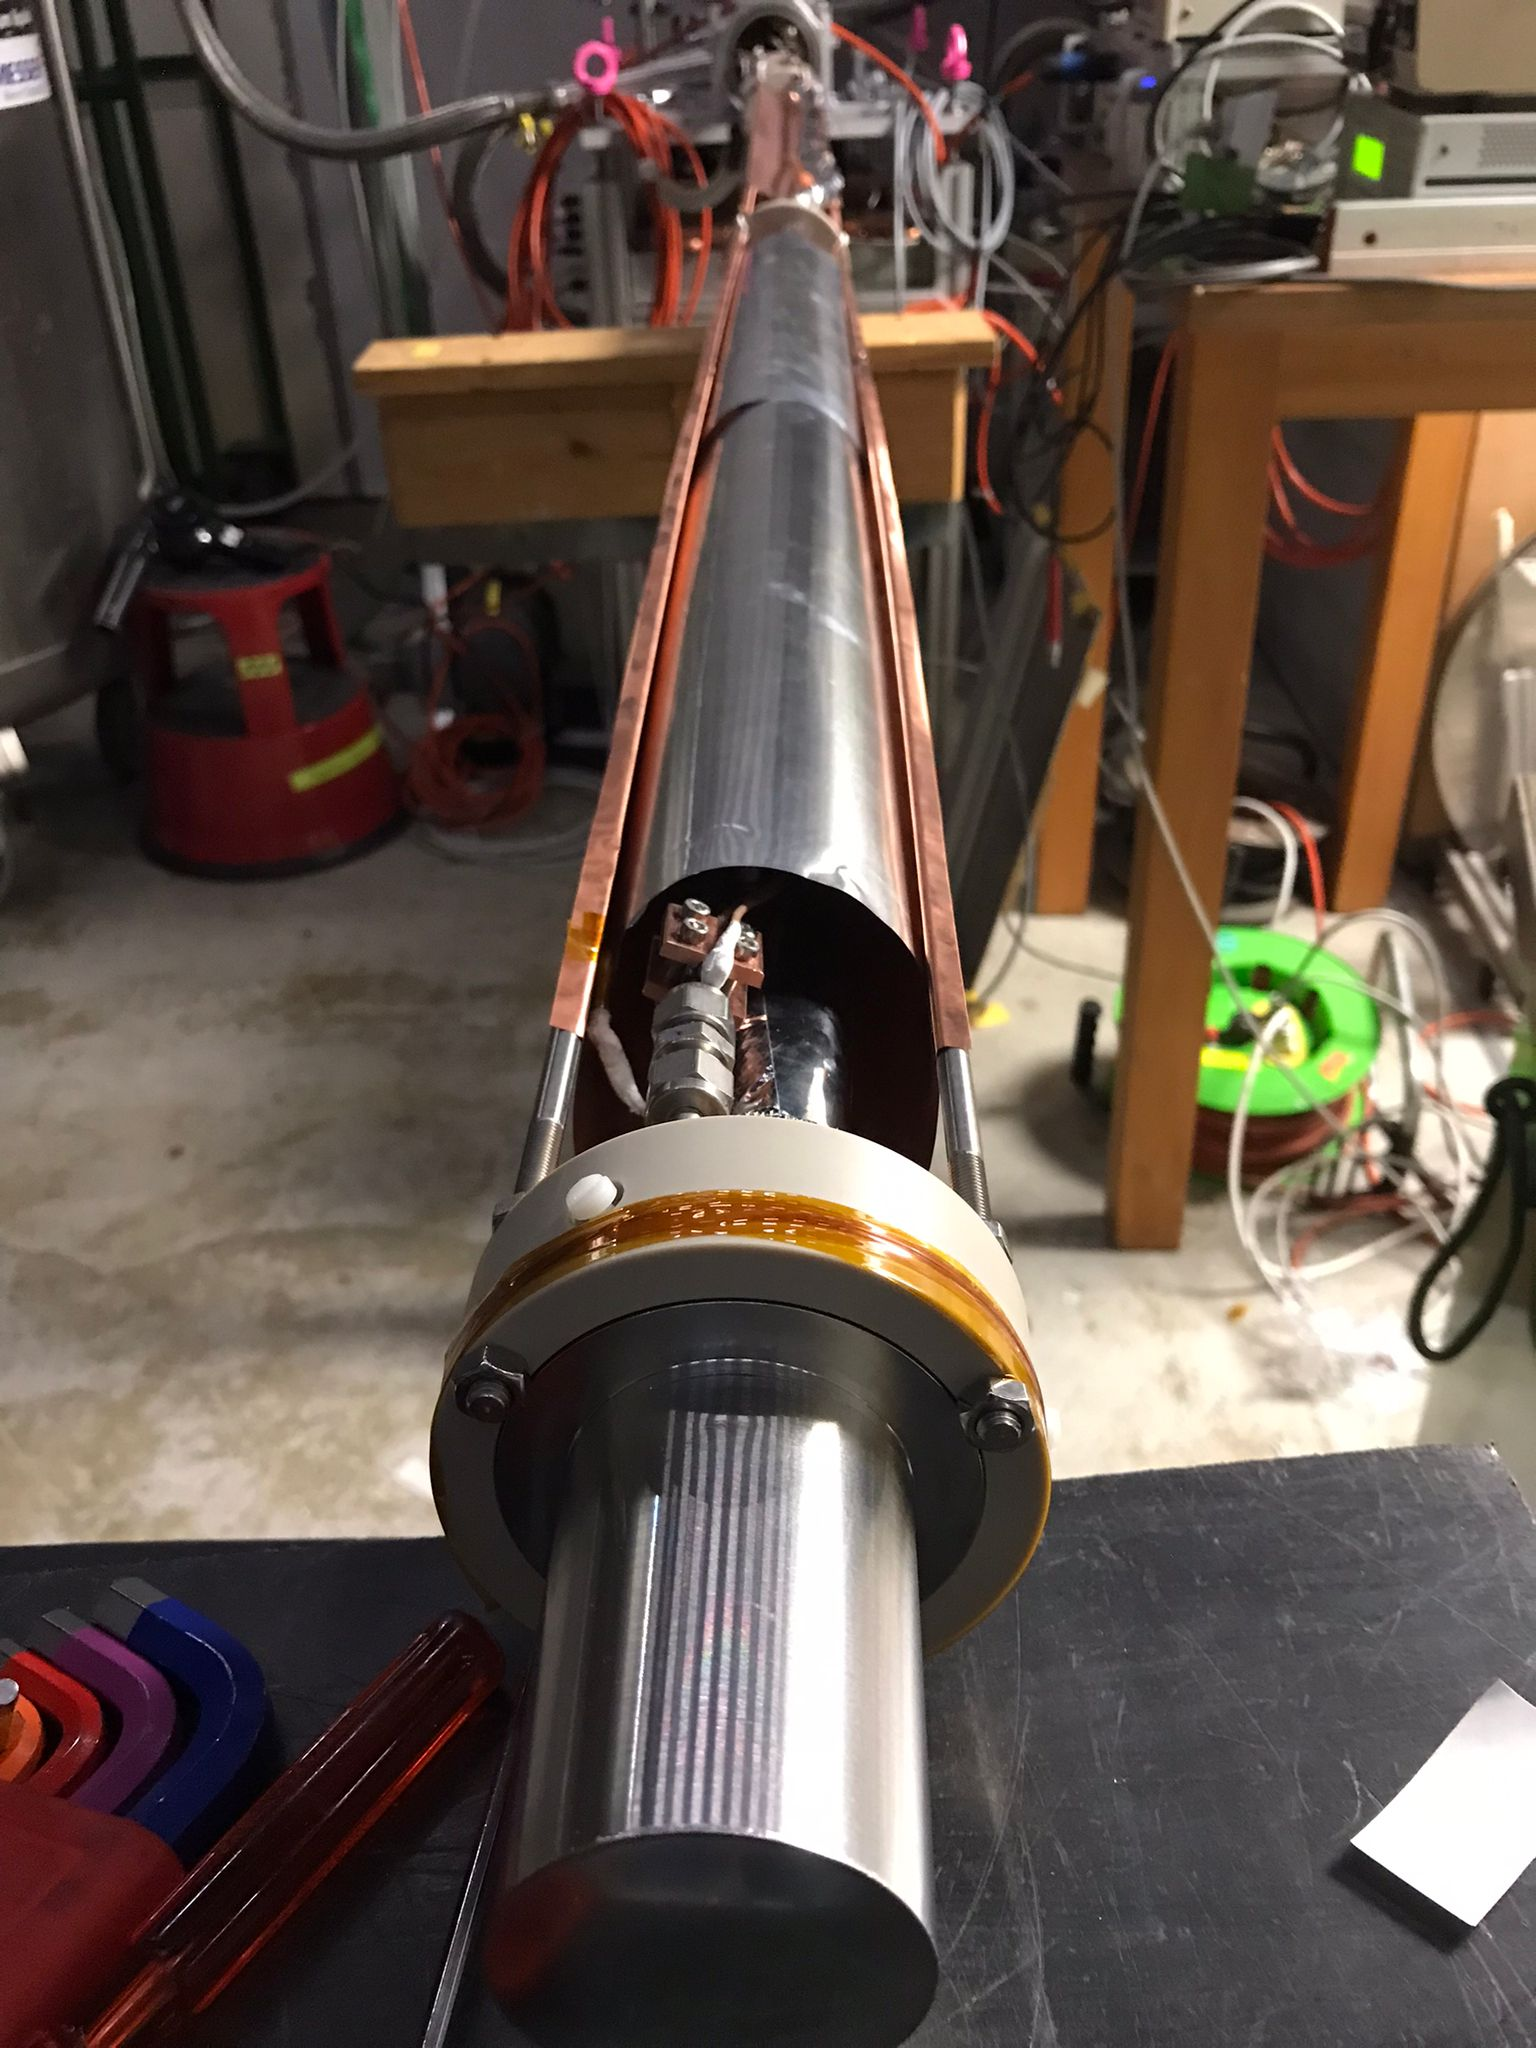
\includegraphics[height = 10cm, keepaspectratio]{Figures/LH2/2022/CEX2022_shielding.jpeg}}
            \caption{Picture of the improved heat shielding of the system. The multi-layer super insulation was added to the Cu rod (a) the outlet was designed to be under vacuum and with a nozzle of a transferring line for He (b) and the copper shielding of the whole target can be seen in (c).}
            \label{fig:CEX:2022:insulation}
        \end{figure}
        
    \status{review}
    \subsection{Data taking}
        The 2022 data taking was similar in structure to the previous: roughly two weeks of CR and CEX runs alternated given the status of the target.
        CEX data were collected when the target was considered `full enough': below 2.1 bar, meaning 50\% full. 
        In the two weeks, this translates to efficiency of $D_{2021}\approx0.6$.
        The hydrogen and helium pressure during data-taking is shown in Fig.~\ref{fig:CEX:datataking:2022}.
        The efficiency for 2022 was higher than the previous year and was enough to collect the necessary statistics for every patch (Fig.~\ref{fig:CEX:patches:2022}).
        The analysis of the data collected during 2022 is still ongoing.

\status{review}
\section{2023}
    Although the 2022 CEX campaign was much more successful than the previous one, the limitations of the second iteration dictated a hectic schedule during data taking. 
    The (somewhat risky) modification of the liquid hydrogen cup turned out to be a good improvement but there was still room for refinement. 
    Mainly, we wanted to reduce the time/amount of liquid Helium needed to reach the liquid hydrogen status. 
    For this reason, we went back to the drawing board.
    The starting idea of the design used in 2021 and 2022 was to assess the feasibility of using a long Cu rod to transport the heat with the final aim of installing a 'cold head' as a cooling mechanism.
    This system was proven good enough for the calibrations needed but eventually, the re-design of the system was deemed unnecessary.
    Once the plan of installing a cryopump was no longer on the table, we opted to adapt the current design free from the constraint of having such a long system. 

    \status{review}
    \subsection{Upgrade}
        \paragraph{He circuit}
        The first item was to try reducing the time needed to cool the system down.
        In this direction, the only change on the Helium circuit was to install a new cooling coil.
        This was built in a similar fashion but longer (\SI{120}{mm} instead of \SI{60}{mm}) increasing the thermal conduction between liquid helium and the main copper parts.
        A sketch of the new copper coil is shown in Fig.~\ref{fig:}.
        On top of this change to the He circuit, we replaced the copper rod with a shorter copper cylinder, threaded on both sides, to reduce the thermal load of the system.
        This meant the position of the cooling coil was moved further inside COBRA, requiring longer in/out helium lines. 
        
        \paragraph{Cell} Learning from the modifications done in 2022, a new Cell was produced (see Fig.~\ref{fig:}):
        \begin{outline}
            \1 This was built with the copper connection so that it could be screwed on the copper rod
            \1 The thermal connection with the copper was improved by making the wall thinner (\SI{-999}{mm} instead of \SI{-999}{mm}) and having a larger copper surface, covering most of the wall (see Fig.~\ref{fig:})
        \end{outline}
        
        \paragraph{Shielding} The shielding also went through few changes:
        \begin{outline}
            \1 Multi-layer insulation was added to the in/out helium lines, to prevent the liquid helium from evaporating before reaching the cooling coil.
            \1 A copper shielding was added around the cooling section
            \1 Multi-layer insulation was added to the cell itself to improve the stability of the system 
        \end{outline}

        \paragraph{Sensors} As already discussed, the slow control of the system is based on an SCS2000.
        Just like in 2022, unfortunately, we did not manage to have the \lakeshore read by this module, meaning they were not recorded on the MIDAS page of the experiment.\\
        In total, we had four \lakeshore sensors:
        \begin{outline}
            \1 Two sensors were placed on the inlet and outlet of the helium line, near the cooler.
            \1 Two were used to follow the temperature of the cell
                \2 one at the end of the Cu rod, to ensure the cooler-rod thermal connection
                \2 one on the cell, to ensure the rod-cell thermal connection 
        \end{outline}
        The sensors are shown in Fig.~\ref{fig:CEX:2023:sensors}.

    \status{review}
    \subsection{Tests}
        A few hiccups with the production and delivery of the parts forced us into a hectic schedule to ensure the proper testing of this renovated system.
        The main challenges were linked to a mistake in the production of the cooler, which led to unwanted thermal connections and the reproducibility of the proper thermal connection when screwing the different parts together.
        The first problem was solved by adjusting the assembly procedure. The second point was solved, with a bit of trial and error, using thermal grease and indium.
        In Fig.~\ref{fig:CEX:2023:tests} the results of one of the successful liquefaction. 
        In the plot, the azure line represents how full the cell is. 
        The reason for the multiple drops is that the test was to reduce the Helium flux while keeping the liquid Hydrogen.

        \begin{figure}[ht]   
            \centering
            \subfloat[The sensor have been placed on the He lines with a Cu `clamp'.]{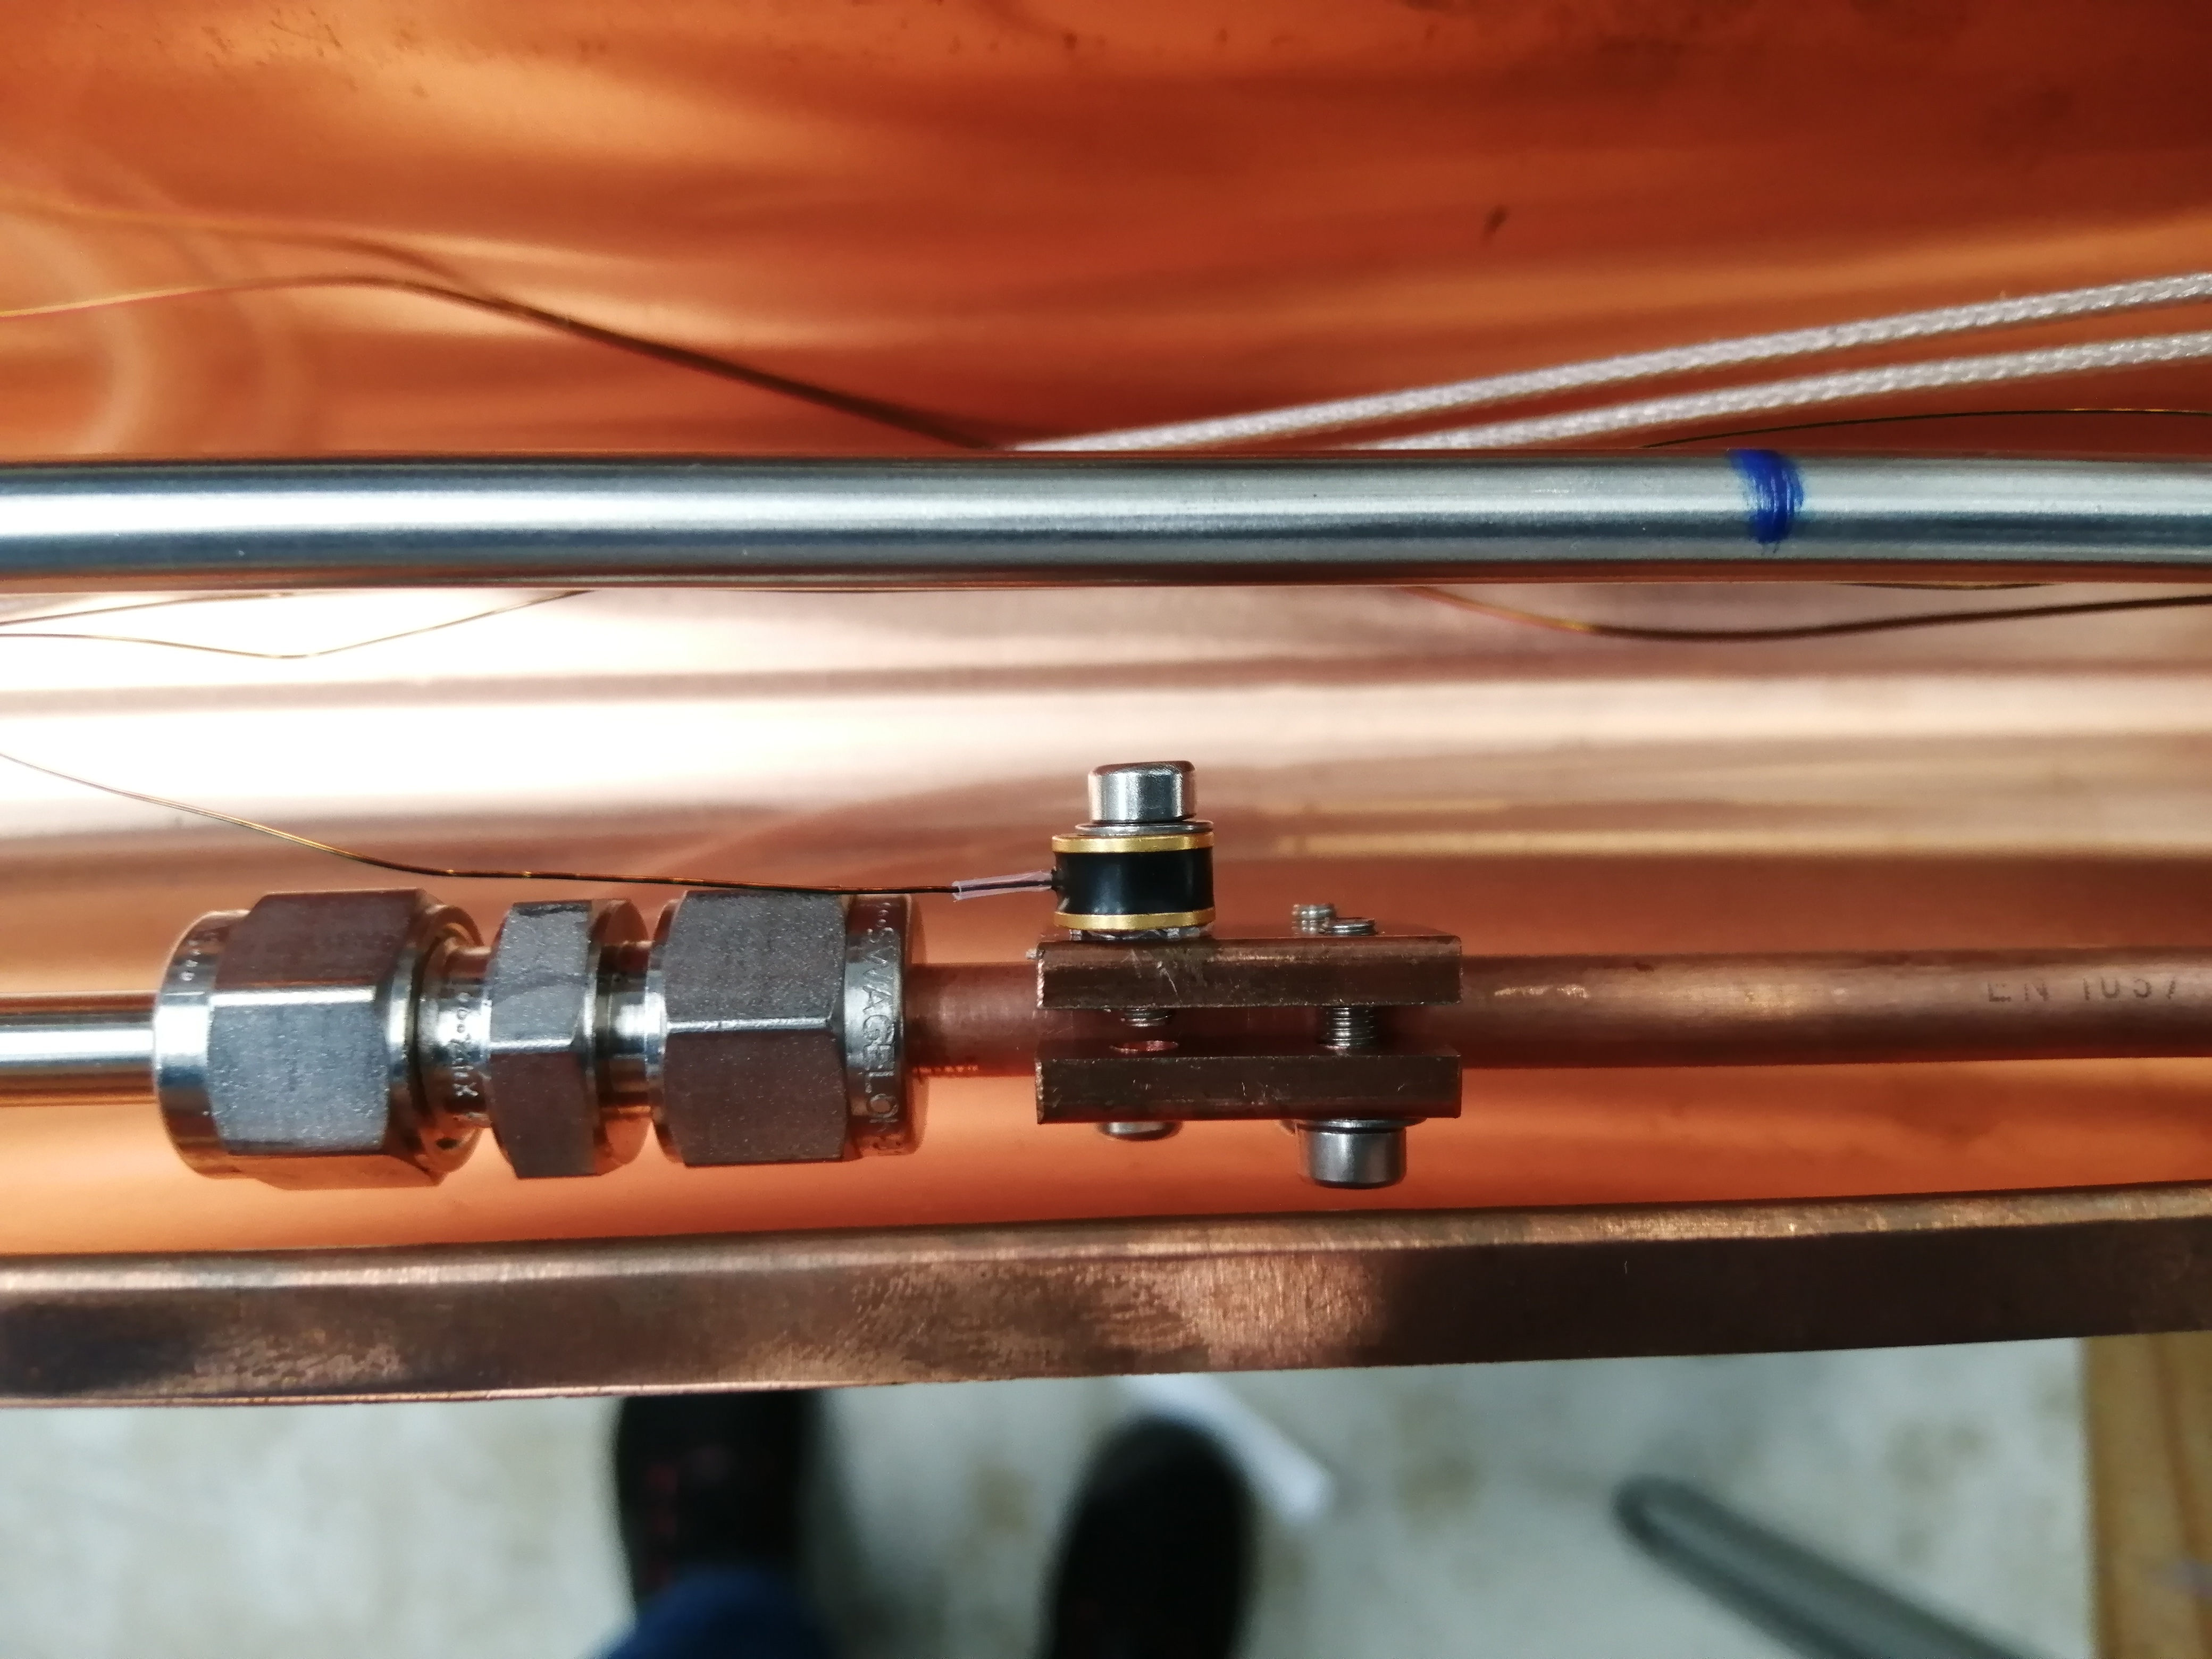
\includegraphics[height = 6cm, keepaspectratio]{Figures/LH2/2023/CEX2023_sensors_inlet.jpg}}
            \hfill
            \subfloat[An additional sensor on the cell to ensure the thermal contact.]{
            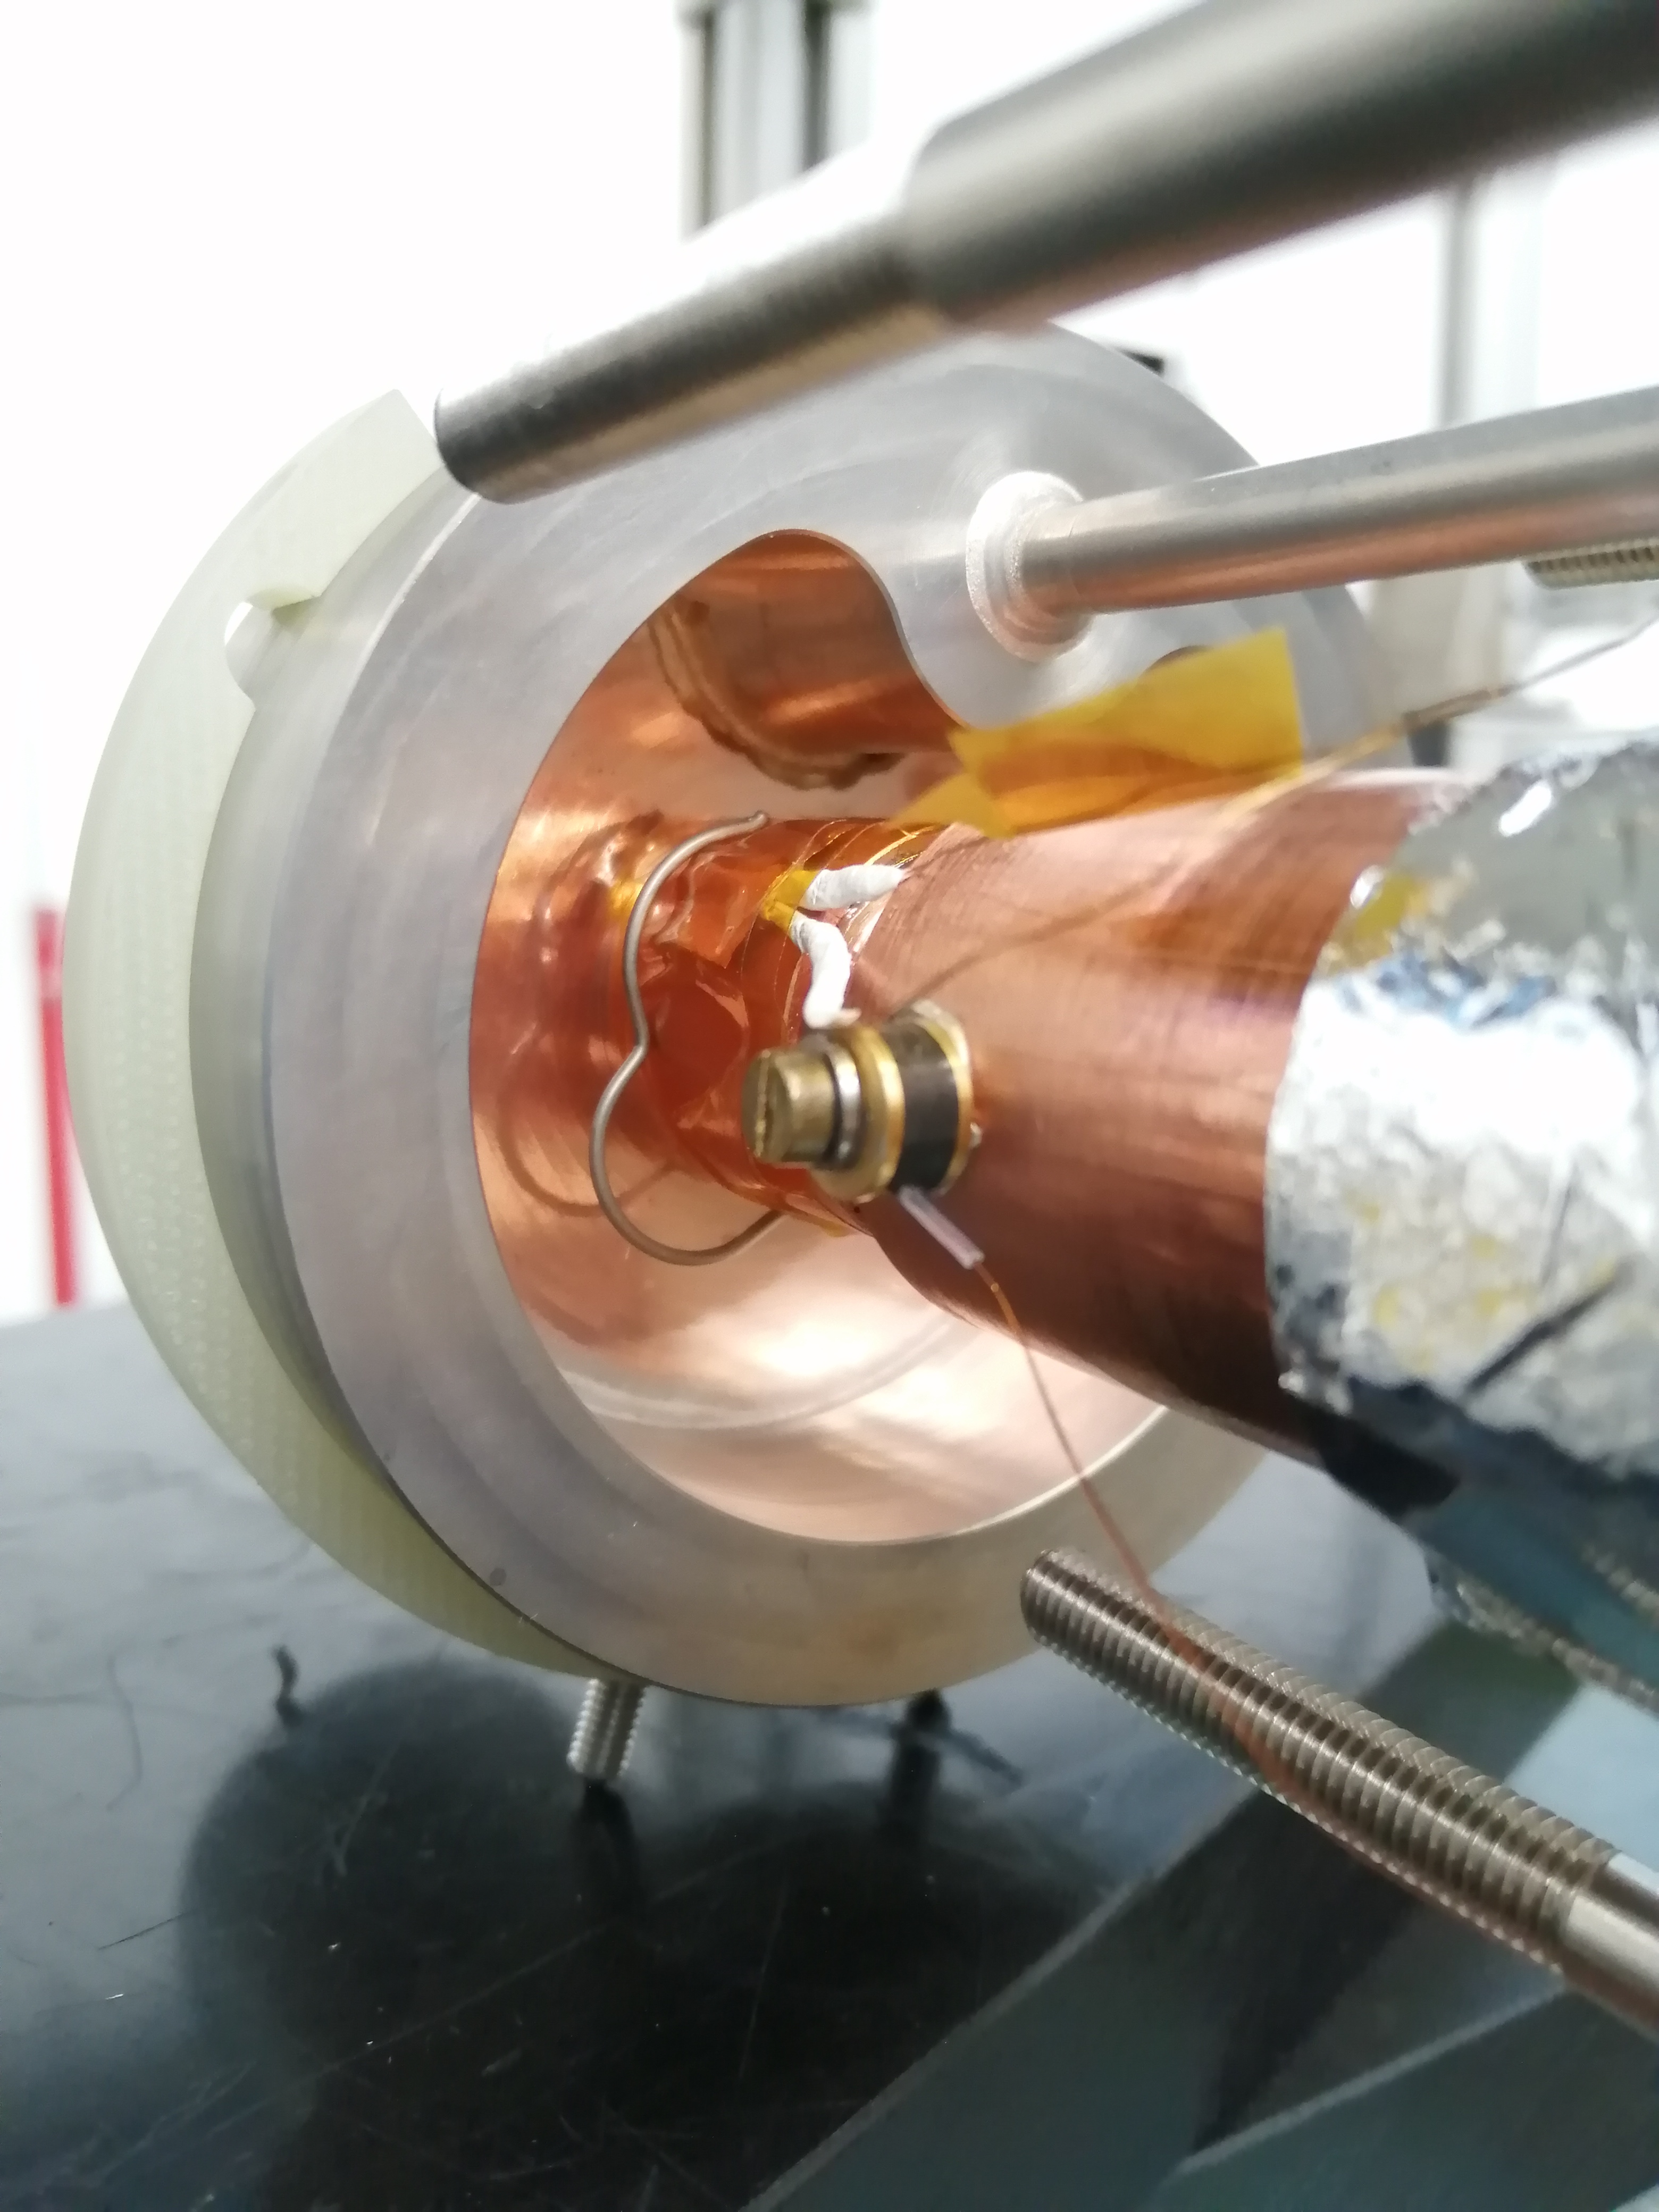
\includegraphics[height = 6cm, keepaspectratio]{Figures/LH2/2023/LH2_cellSensor.jpg}}
            \caption{To study the behaviour and stability of the system, additional \lakeshore sensors were placed on the inlet/outile He lines (a) and both on the CU rod and the cell (b). The additional sensor on the copper part of the cell, although not easy to place, allowed us to ensure the thermal connection.}
            \label{fig:CEX:2023:sensors}
        \end{figure}

        \begin{figure}[ht]   
            \centering
            \subfloat[Picture of the `compact' \ce{LH2}.]{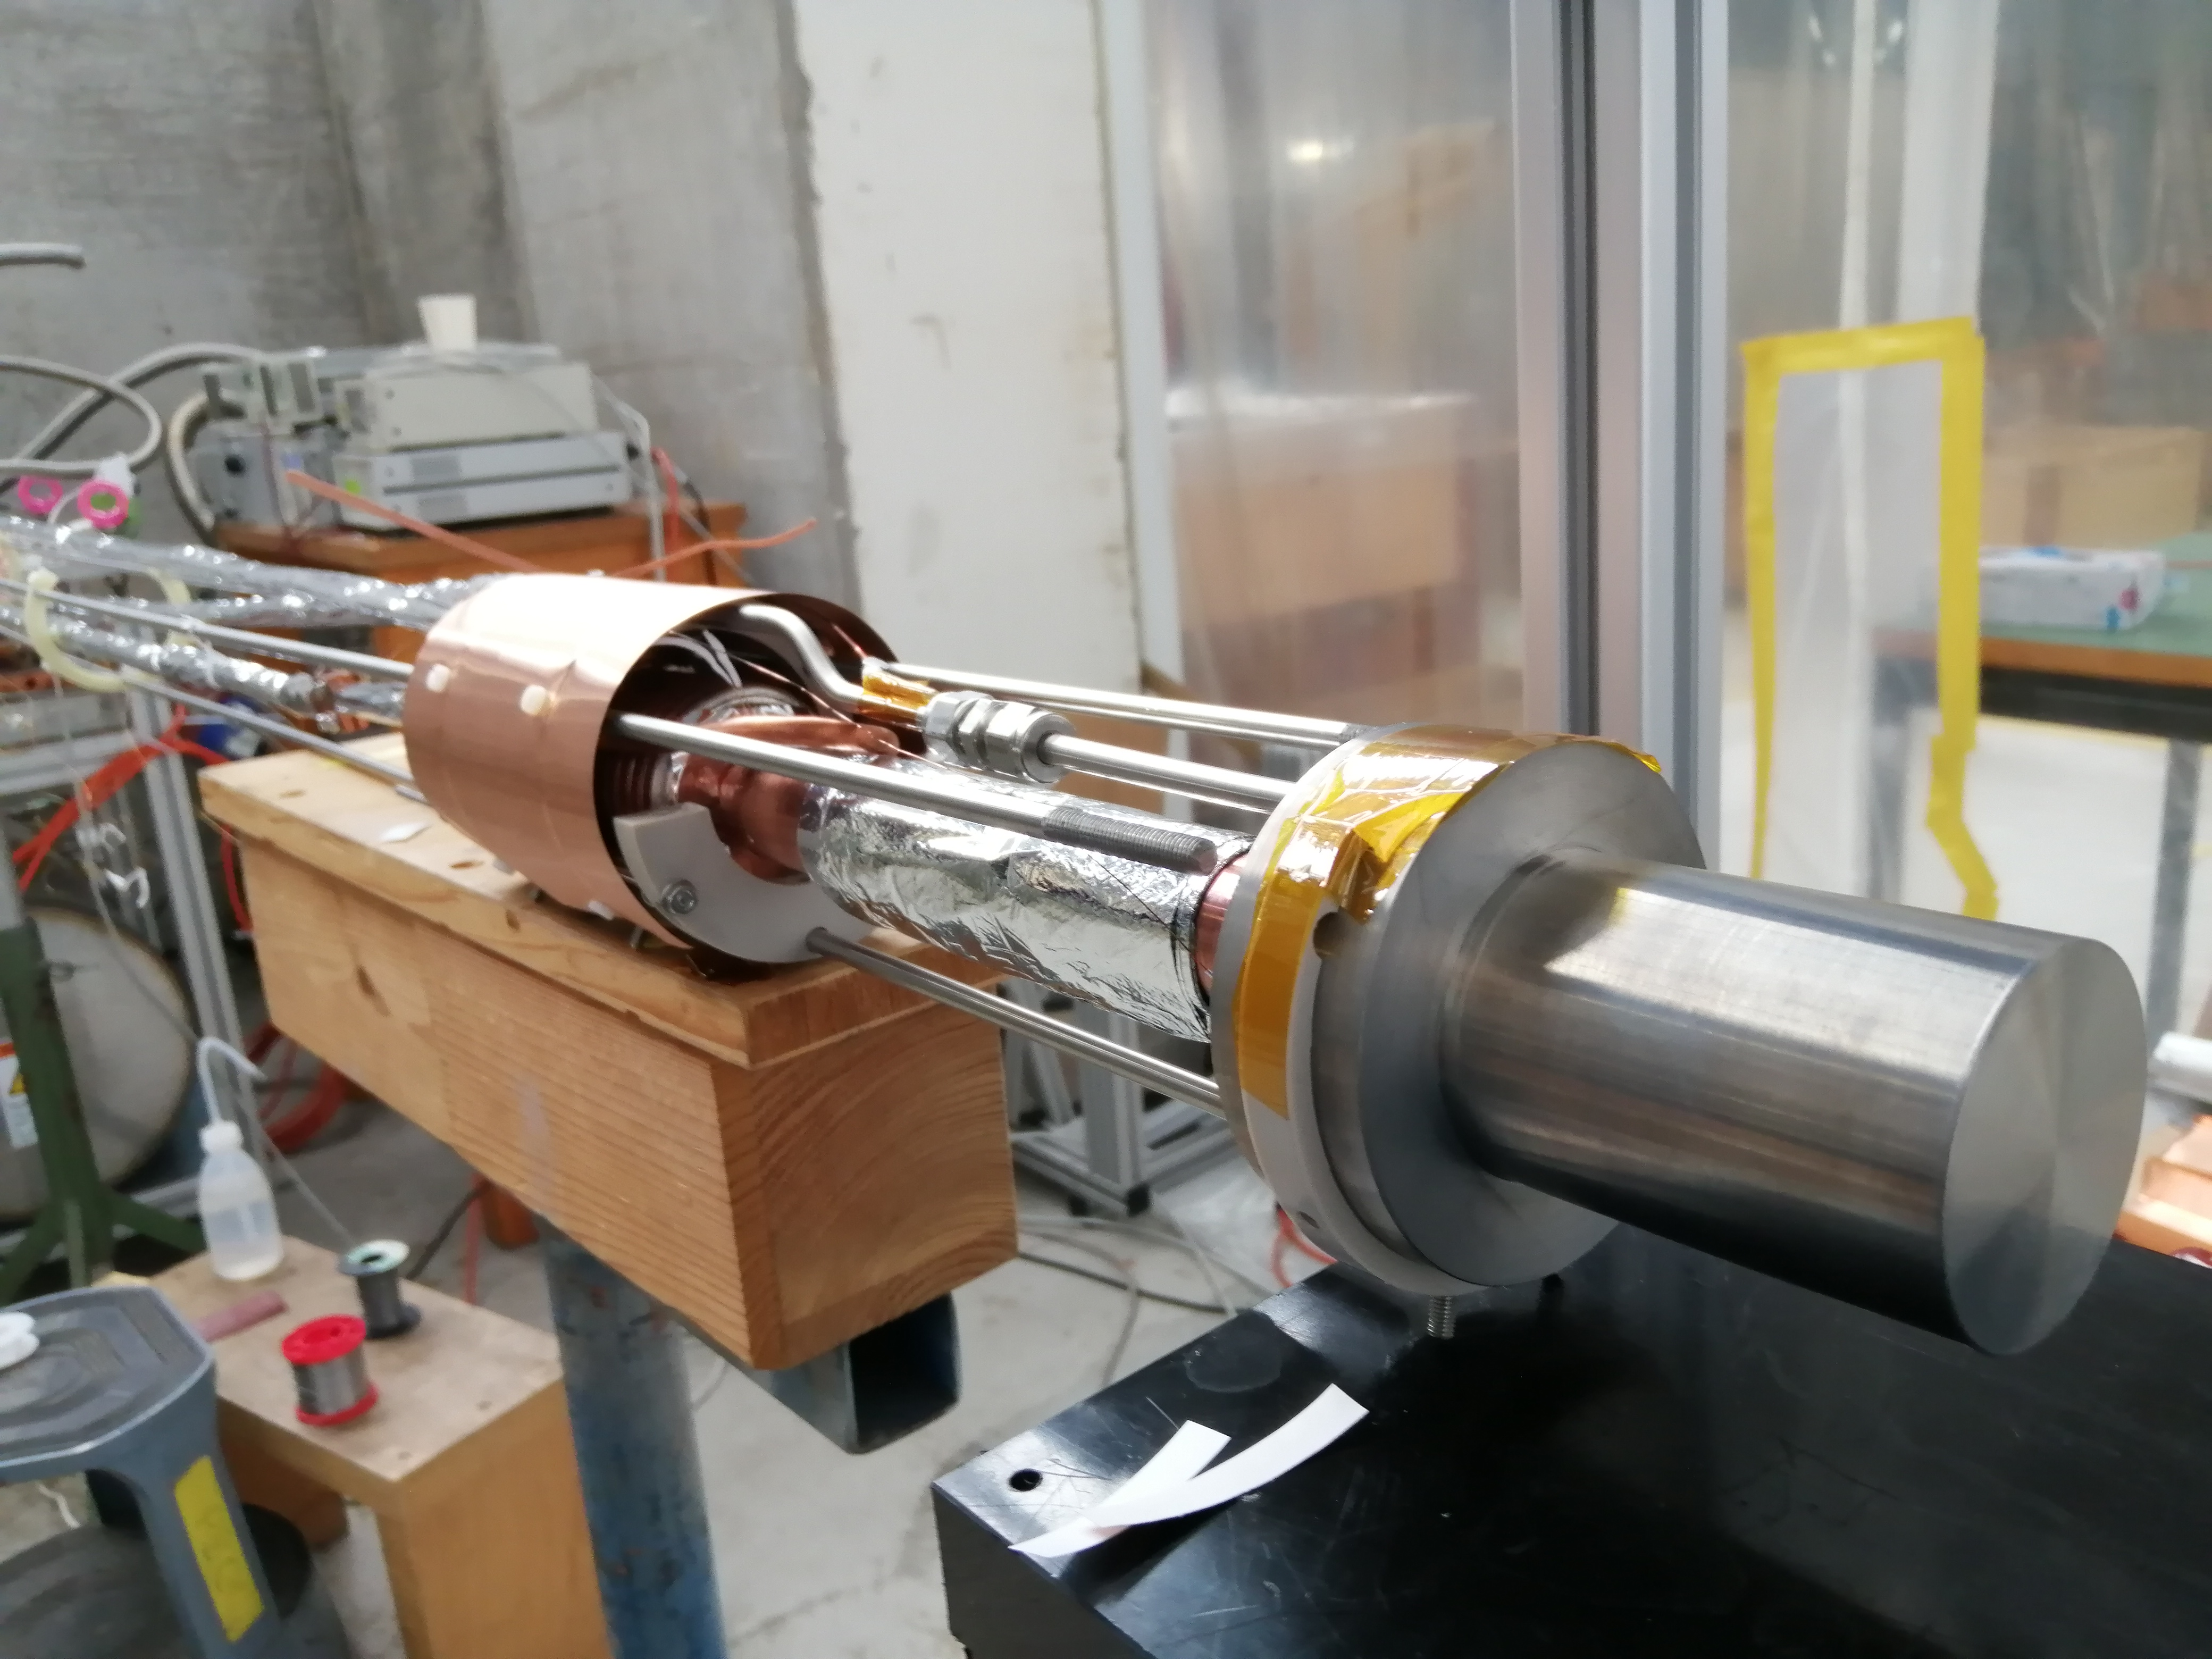
\includegraphics[height = 6cm, keepaspectratio]{Figures/LH2/2023/LH2_compact.jpg}}
            \hfill
            \subfloat[Super-insulation added on the cell.]{
            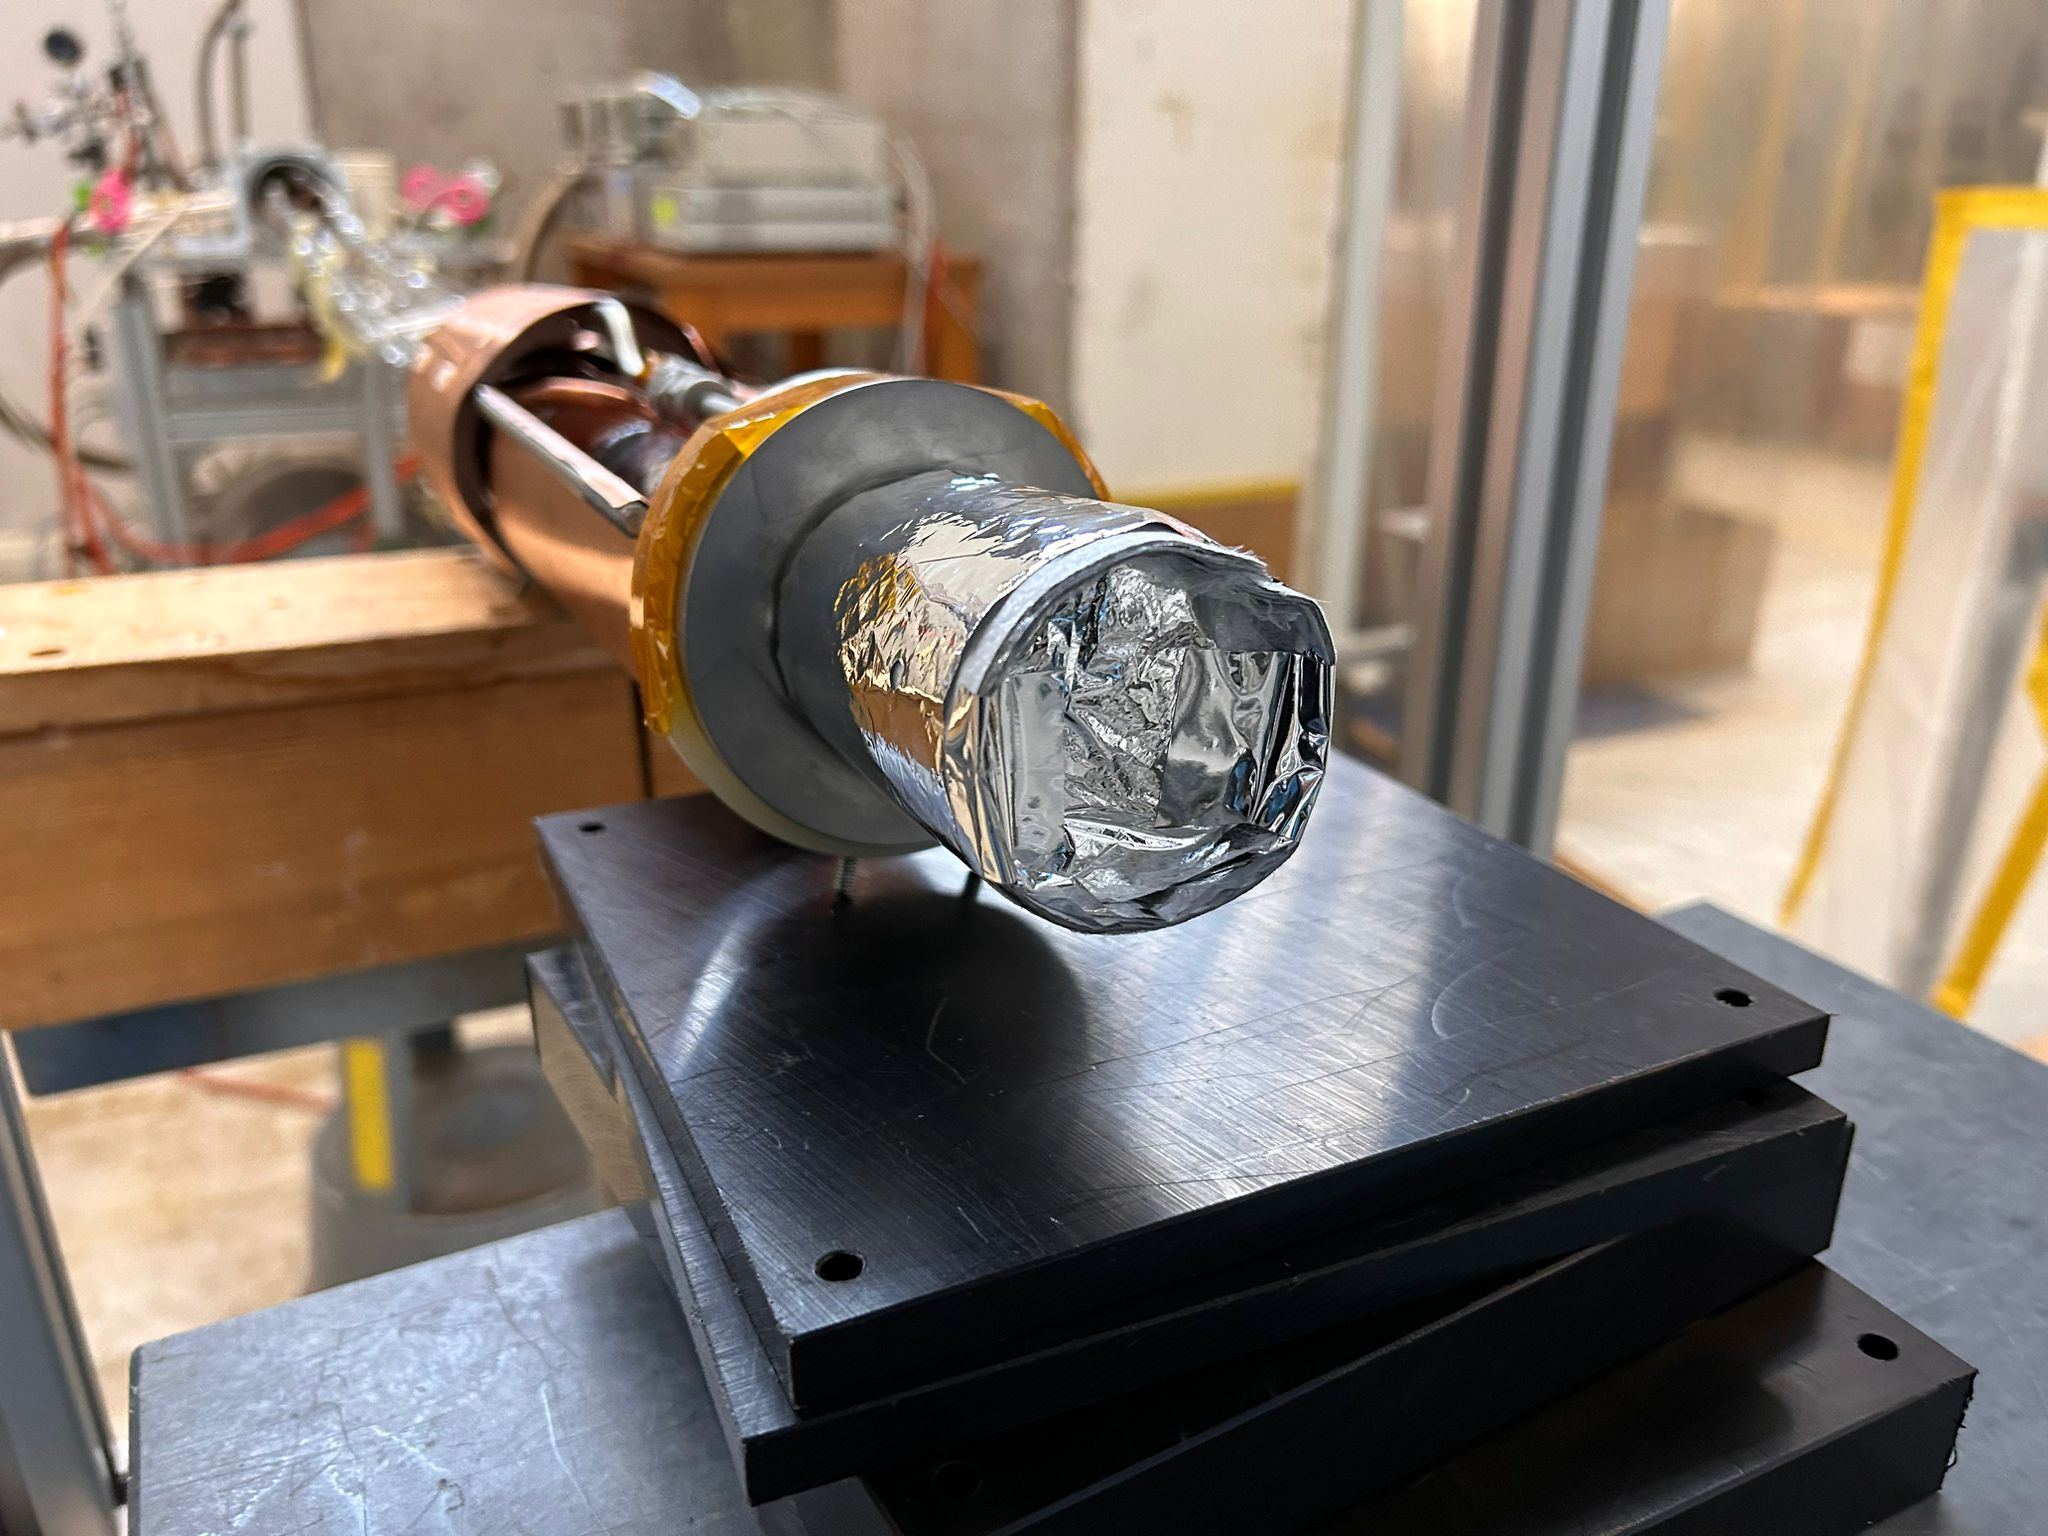
\includegraphics[height = 6cm, keepaspectratio]{Figures/LH2/2023/LH2_cellMLI.jpeg}}
            \caption{The `compact' version of the \ce{LH2} target is shown in (a), with the Cu shield on the cooler, the new vetronite parts and the super-insulation on the different sections. An additional layer of super-insulation was placed on the cell itself (b) to reduce the heat-lode due to radiation of the vacuum pipe.}
            \label{fig:CEX:2023:target}
        \end{figure}
        
        \begin{figure}[ht]   
            \centering
            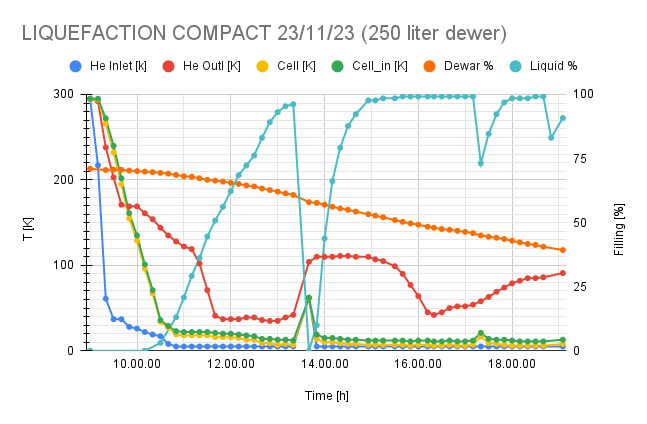
\includegraphics[width=\textwidth, keepaspectratio]{Figures/LH2/2023/LIQUEFACTION_23.11.23(250L).png}
            \caption{This plot illustrates the outcome of a successful liquefaction process. The azure line depicts the fill level of the cell. The repeated drops in the line signify that the test aimed to decrease the Helium flux while maintaining the presence of liquid Hydrogen.}
            \label{fig:CEX:2023:tests}
        \end{figure}
    
    \status{review}
    \subsection{Data taking}
        The last test outside the experimental area was performed on the 13th Oct. 2023 and the target was installed on the 14th.
        The warped shape of the insertion system forced us to insert the target lower than the beam height. 
        After managing a sufficient alignment in \textbf{x} and \textbf{z}, the target was lifted to center it vertically (\textbf{y}). The alignment, shown in Fig.~\ref{fig:CEX:2023:allignement} was performed by observing the tip of the target via the UCI camera (this item was discussed in Sec.~\ref{sec:MEG:target})
        The main points of this data taking were the following:
        \begin{outline}
            \1 The cell was full (>90\%) during data taking. This was unfortunately not the case in 2021 and 2022, during which we collected data when the level was >50\%
            \2[->] Higher trigger rate ($30\ra45$Hz) and better quality events, improvement of $>\times1.5$
            \1 A shorter dead time after the dewar exchange: 30 mins for cooling and 2h for liquefaction
            \2[->] Higher duty-cycle $15\ra20h/24h$, an improvement of $\times1.3$
            \1 We used a 250L dewar every 24h
            \2[->] Cheaper than last year and simpler to organize
        \end{outline}
        Compared to the previous years, more data were collected in a shorter period (Fig.~\ref{fig:CEX:patches:2023}), marking a success for this iteration of the LH2 target. 
        At the same time, the usage of Liquid Helium, although still elevated, was much lower than in 2022. In Fig.~\ref{fig:CEX:dewar} the comparison between the dewar usage in 2022 and 2023 (this info was lost for 2021).
        The analysis of the data collected is still ongoing.

        \begin{figure}
            \centering
            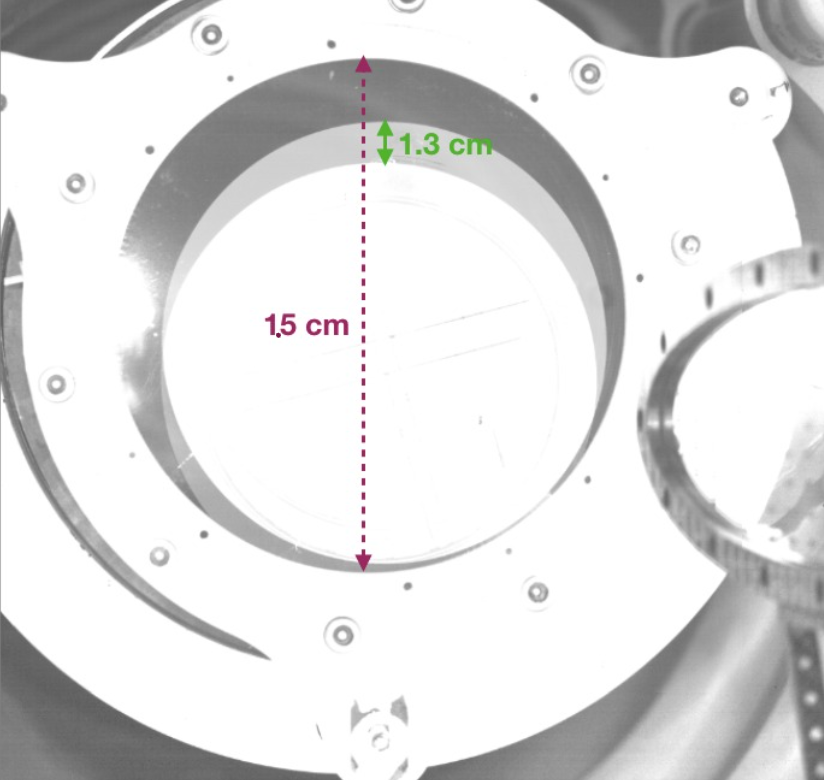
\includegraphics[width=0.6\textwidth]{Figures/LH2/2023/LH2_UCI_2023.png}
            \caption[Short Caption]{After inserting the target in COBRA, it was centered (as much as possible). In red a known distance for reference, in green the displacement needed to center it. NB: the UCI pictures are upside-down.}
            \label{fig:CEX:2023:allignement}
        \end{figure}

        \begin{figure}
            \centering
            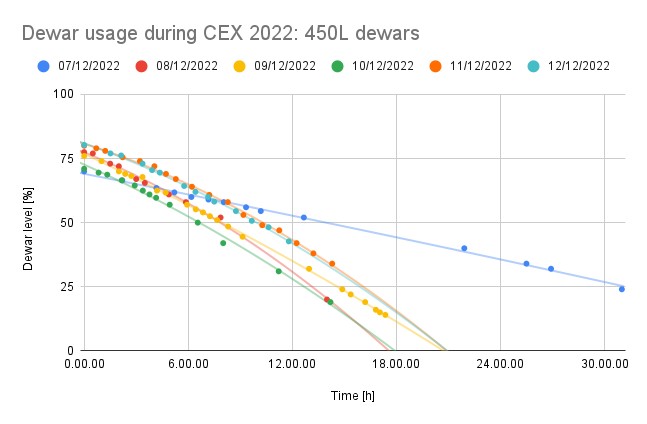
\includegraphics[width=0.9\textwidth, keepaspectratio]{Figures/LH2/2022/CEX2022_dewars.png}
            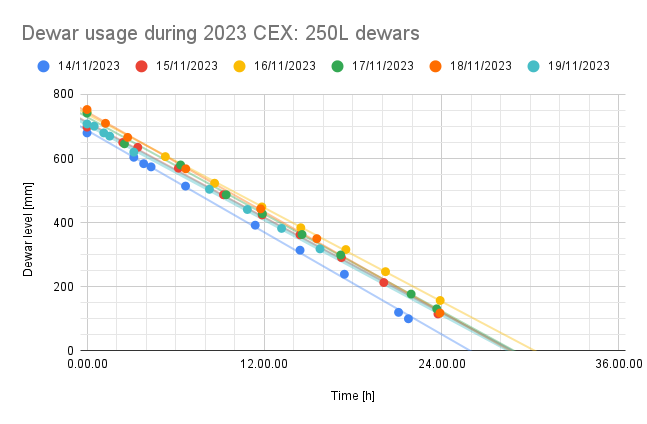
\includegraphics[width=0.9\textwidth, keepaspectratio]{Figures/LH2/2023/2023CEX_dewars.png}
            \caption[Dewar usage in 2022 and 2023.]{Comparison of the dewar usage in 2022 and 2023. While the general trend during 2023 has been much better than in 2022, a spurious day of data-taking in 2022 was particularly efficient. The reason is unfortunately no clear and the condition hard to reproduce.}
            \label{fig:CEX:dewar}
        \end{figure}

    \begin{figure}[ht]   
            \centering
            \subfloat[CEX2021]{
            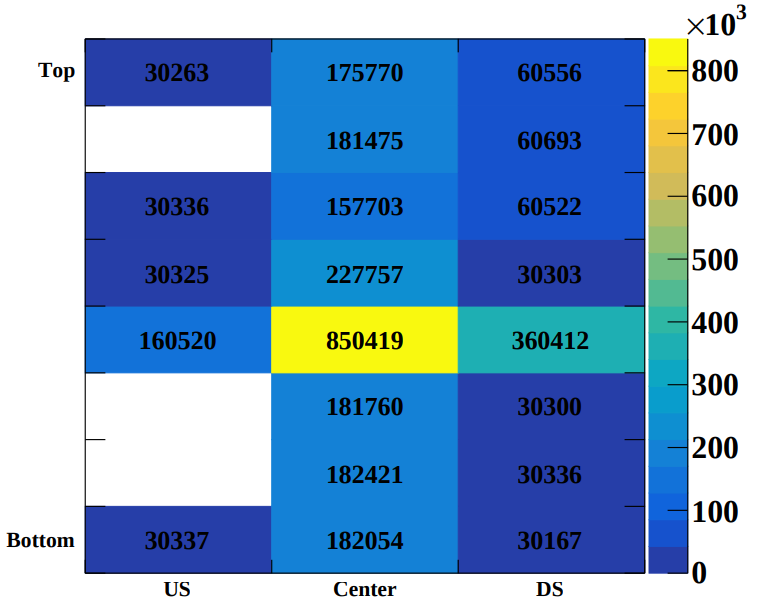
\includegraphics[height = 6cm, keepaspectratio]{Figures/LH2/2021/CEX2021_patches.png}            \label{fig:CEX:patches:2021}}
            \hfill
            \subfloat[CEX2022]{
            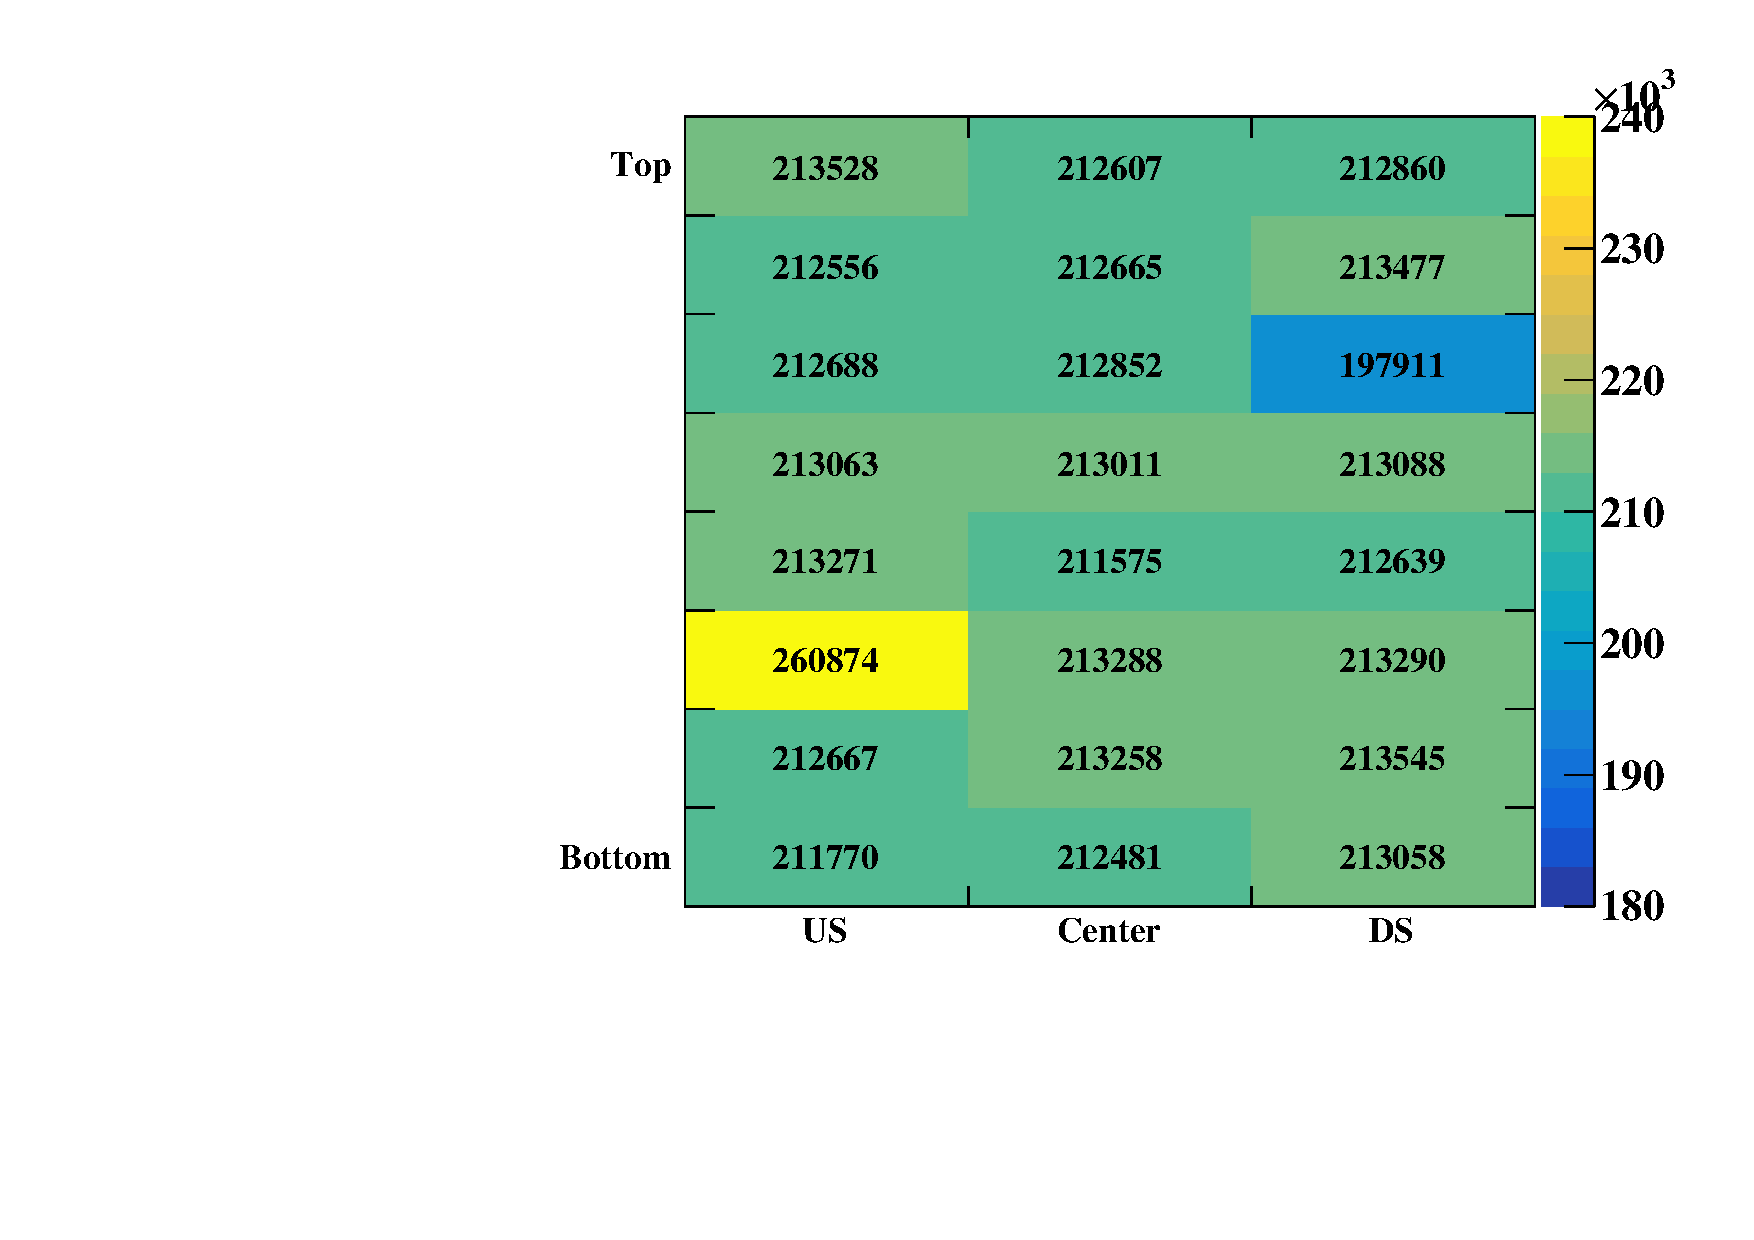
\includegraphics[height = 6cm, keepaspectratio]{Figures/LH2/2022/CEX2022_patches.pdf}            \label{fig:CEX:patches:2022}}
            \hfill
            \subfloat[CEX2023]{
            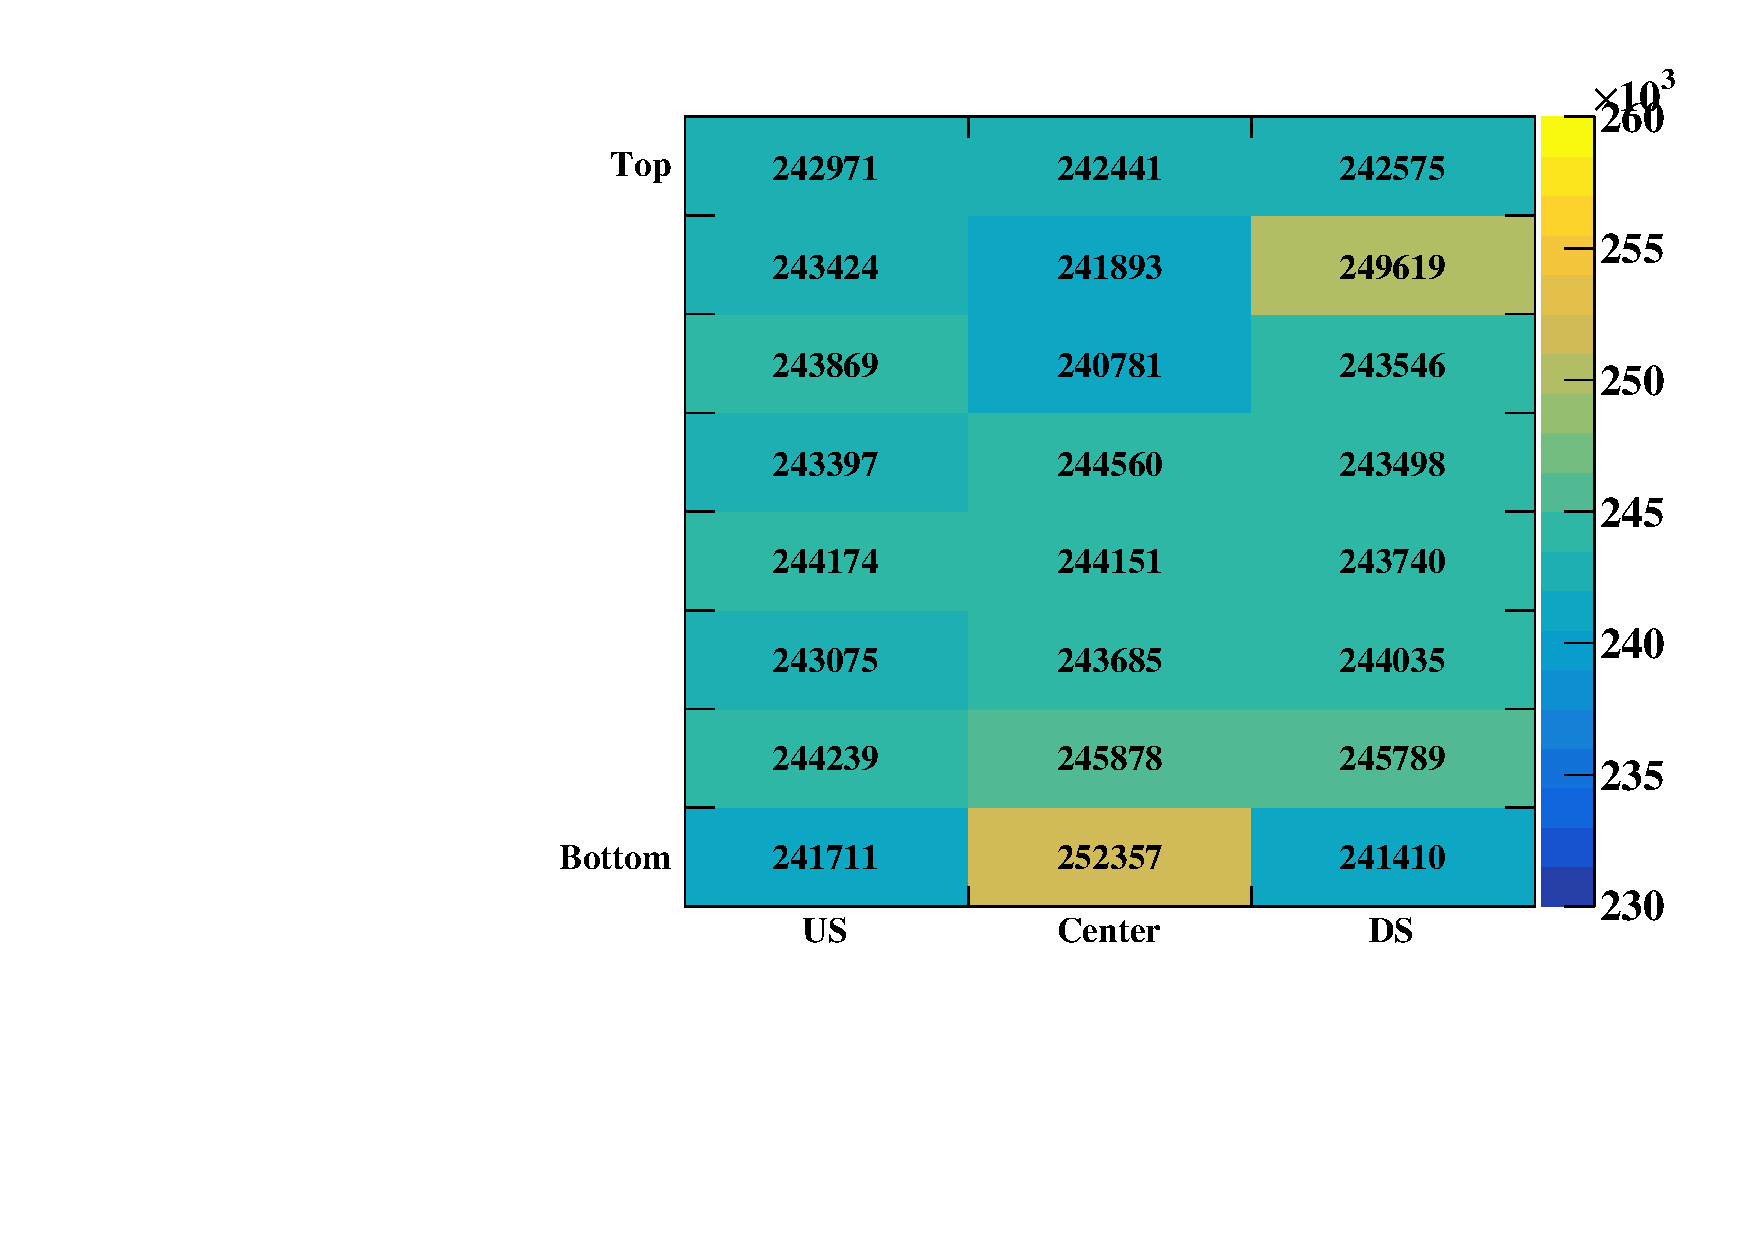
\includegraphics[height = 6cm, keepaspectratio]{Figures/LH2/2023/CEX2023_patches.pdf}            \label{fig:CEX:patches:2023}}
            \caption{Number of triggered events during Charge EXchange data taking in 2021 2022 and 2023. Notice the lack of events in 3 patches in 2021 due to the low dutycycle of the LH2 target. For 2022 and 2023, the required statistics was collected and exceeded.}
            \label{fig:CEX:patches}
        \end{figure}

\status{review}
\section{Conclusions}
    After a recap of the task at hand, the history of the Hydrogen Target design was highlighted. As just illustrated, the duty cycle, the stability, and the level of the target improved significantly during these three years: $D_{2021, 50\%}\approx 0.55 \ra D_{2022, 50\%}\approx0.6 \ra D_{2023, 90\%}>0.8$. Although minor adjustments are still planned, this will probably stay as the final design.\\


    \begin{figure}[ht]   
    \centering
        \subfloat[CEX 2021: beam below \SI{2.1}{bar}. 
        This translates to a duty cycle of $D_{2021}\approx0.5$,  with target level $>50\%$. 
        The low efficiency prevented the collection of the necessary statistics for every patch.]{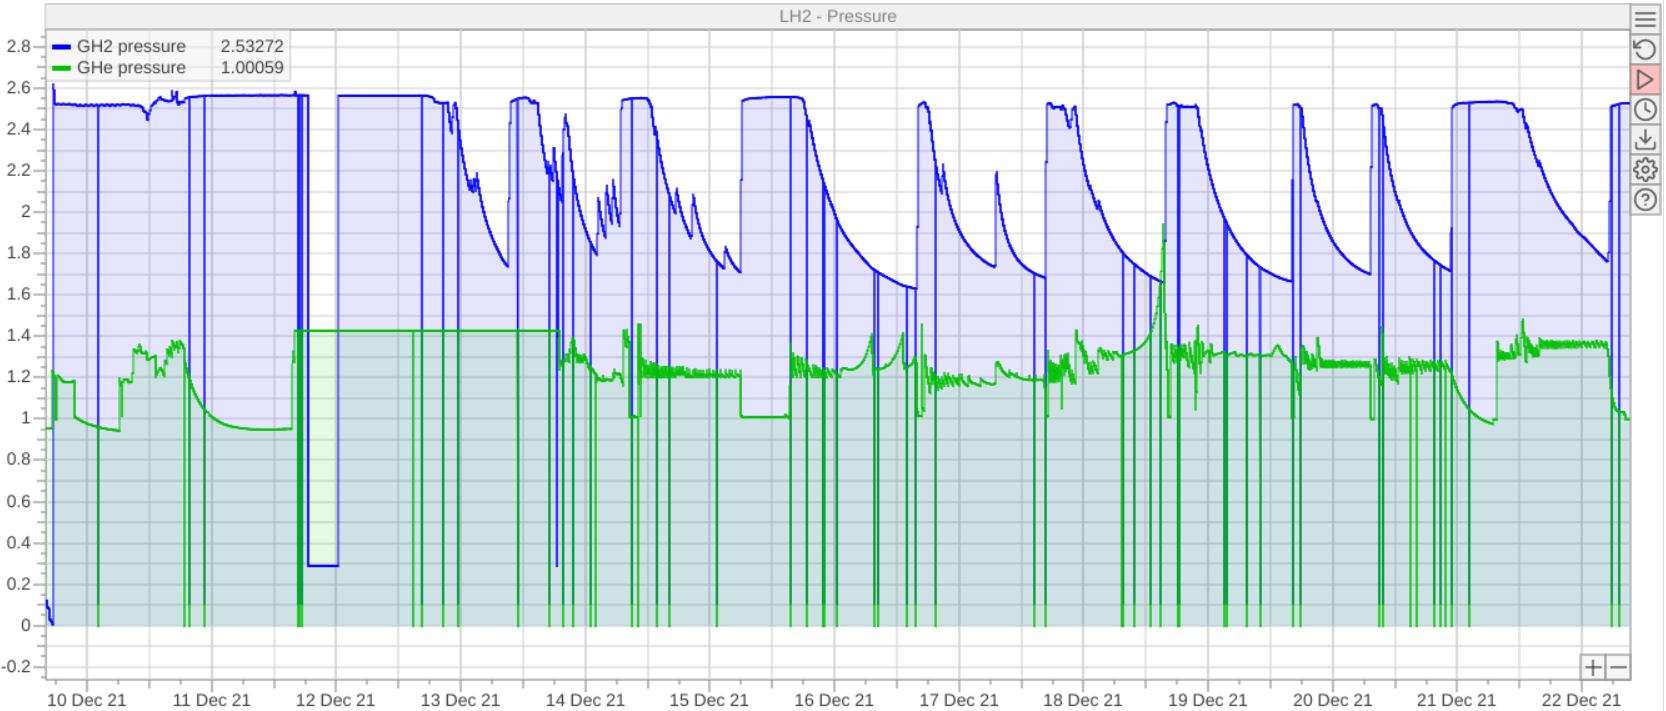
\includegraphics[width=0.9\textwidth, height=6cm]{Figures/LH2/2021CEX_LH2.png}\label{fig:CEX:datataking:2021}}\\
        \subfloat[CEX 2022: beam below \SI{2.1}{bar}. 
        This translates to a duty cycle of $D_{2022}\approx0.6$, with target level $>50\%$.]{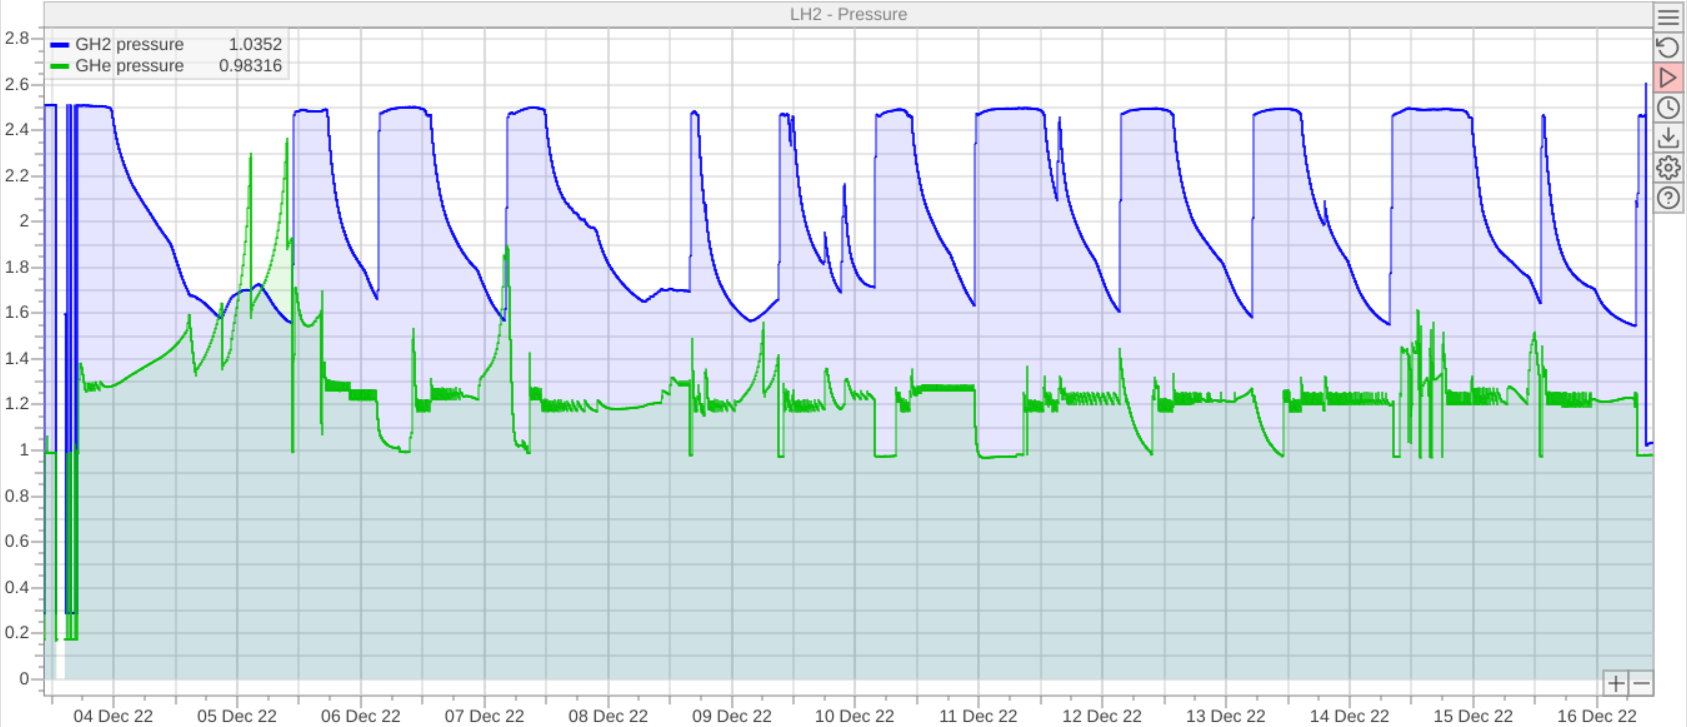
\includegraphics[width=0.9\textwidth, height=6cm]{Figures/LH2/2022CEX_LH2.png}\label{fig:CEX:datataking:2022}}\\
        \subfloat[CEX 2023: beam below \SI{1.9}{bar}. 
        This translates to a duty cycle of $D_{2023}>0.8$, with target level $>90\%$.]{
        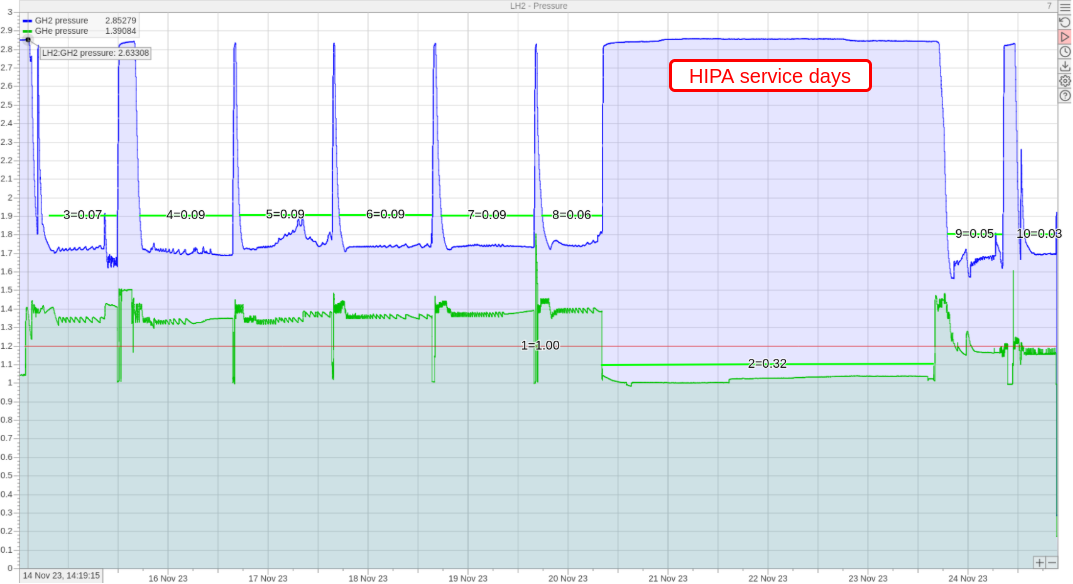
\includegraphics[width=0.9\textwidth, height=6cm]{Figures/LH2/2023CEX_LH2.png}\label{fig:CEX:datataking:2023}}
        \caption{Measured hydrogen pressure in the target and helium pressure in the dewar used for cooling during the different CEX data takings. 
        The beam was ON (red line) when the target was considered `full enough'. This value changed as a consequence of the different upgrades of the target and was evaluated by measuring the XEC trigger rate.}
        \label{fig:CEX:datataking}
    \end{figure}

    \noindent
    The development of this system has been my first (and only) real immersion in the vast subject of cryogenics. 
    Many things were quite new to me, from the materials' thermal properties to the inner structure of a Helium dewar and from the working principle of low-temperature sensors to the CAD design of peek/vetronite parts required for structural stability and thermal insulation.
    Although being still far from any shade of \textit{expertise}, this has been quite an eye-opening endeavor.
    
\status{started}
\printbibliography[
    heading = bibliographychapter,
    title=Bibliography on \ce{LH2}
]

\end{refsection}
